%&preformat-present

\newif\ifpresentation % Условие, проверяющее, что документ --- презентация
\presentationtrue
\documentclass[10pt, xcolor={dvipsnames, table, hyperref}]{beamer}

% Новые переменные, которые могут использоваться во всём проекте
% ГОСТ 7.0.11-2011
% 9.2 Оформление текста автореферата диссертации
% 9.2.1 Общая характеристика работы включает в себя следующие основные структурные
% элементы:
% актуальность темы исследования;
\newcommand{\actualityTXT}{Актуальность темы.}
% степень ее разработанности;
\newcommand{\progressTXT}{Степень разработанности темы.}
% цели и задачи;
\newcommand{\aimTXT}{Целью}
\newcommand{\tasksTXT}{задачи}
% научную новизну;
\newcommand{\noveltyTXT}{Научная новизна:}
% теоретическую и практическую значимость работы;
%\newcommand{\influenceTXT}{Теоретическая и практическая значимость}
% или чаще используют просто
\newcommand{\influenceTXT}{Практическая значимость}
% методологию и методы исследования;
\newcommand{\methodsTXT}{Методология и методы исследования.}
% положения, выносимые на защиту;
\newcommand{\defpositionsTXT}{Основные положения, выносимые на~защиту:}
% степень достоверности и апробацию результатов.
\newcommand{\reliabilityTXT}{Достоверность}
\newcommand{\probationTXT}{Апробация работы.}

\newcommand{\contributionTXT}{Личный вклад.}
\newcommand{\publicationsTXT}{Публикации.}


%%% Заголовки библиографии:

% для автореферата:
\newcommand{\bibtitleauthor}{Публикации автора по теме диссертации}

% для стиля библиографии `\insertbiblioauthorgrouped`
\newcommand{\bibtitleauthorvak}{В изданиях из списка ВАК РФ}
\newcommand{\bibtitleauthorscopus}{В изданиях, входящих в международную базу цитирования Scopus}
\newcommand{\bibtitleauthorwos}{В изданиях, входящих в международную базу цитирования Web of Science}
\newcommand{\bibtitleauthorother}{В прочих изданиях}
\newcommand{\bibtitleauthorconf}{В сборниках трудов конференций}

% для стиля библиографии `\insertbiblioauthorimportant`:
\newcommand{\bibtitleauthorimportant}{Наиболее значимые \protect\MakeLowercase\bibtitleauthor}

% для списка литературы в диссертации и списка чужих работ в автореферате:
\newcommand{\bibtitlefull}{Список литературы} % (ГОСТ Р 7.0.11-2011, 4)

\newcommand{\ProgModule}{ПМ АПНДВ} % Название программного модуля

\newcommand\diag[4]{%
    \multicolumn{1}{p{#2}|}{
        \hskip-\tabcolsep
        $\vcenter{
            \begin{tikzpicture}[baseline=0,anchor=south west,inner sep=#1]
                \path[use as bounding box] (0,0) rectangle (#2+2\tabcolsep,\baselineskip);
                \node[minimum width={#2+2\tabcolsep},minimum height=\baselineskip+\extrarowheight] (box) {};
                \draw (box.north west) -- (box.south east);
                \node[anchor=south west] at (box.south west) {#3};
                \node[anchor=north east] at (box.north east) {#4};
            \end{tikzpicture}
        }$\hskip-\tabcolsep
   }
}

\newcommand{\redcell}[1]{
    \cellcolor{red!30} #1 }

\newcommand{\greencell}[1]{
    \cellcolor{green!30} #1 }

\newcommand{\yellowcell}[1]{
    \cellcolor{yellow!30} #1 }

\newcommand{\rpt}[2][1]{%
    \newcounter{loopcntr}
    \forloop{loopcntr}{0}{\value{loopcntr}<#1}{#2}%
  }
            
%%%%%%%%%%%%%%%%%%%%%%%%%%%%%%%%%%%%%%%%%%%%%%%%%%%%%%
%%%% Файл упрощённых настроек шаблона диссертации %%%%
%%%%%%%%%%%%%%%%%%%%%%%%%%%%%%%%%%%%%%%%%%%%%%%%%%%%%%

%%% Инициализирование переменных, не трогать!  %%%
\newcounter{intvl}
\newcounter{otstup}
\newcounter{contnumeq}
\newcounter{contnumfig}
\newcounter{contnumtab}
\newcounter{pgnum}
\newcounter{chapstyle}
\newcounter{headingdelim}
\newcounter{headingalign}
\newcounter{headingsize}
\newcounter{tabcap}
\newcounter{tablaba}
\newcounter{tabtita}
%%%%%%%%%%%%%%%%%%%%%%%%%%%%%%%%%%%%%%%%%%%%%%%%%%%%%%

%%% Область упрощённого управления оформлением %%%

%% Интервал между заголовками и между заголовком и текстом %%
% Заголовки отделяют от текста сверху и снизу
% тремя интервалами (ГОСТ Р 7.0.11-2011, 5.3.5)
\setcounter{intvl}{3}               % Коэффициент кратности к размеру шрифта

%% Отступы у заголовков в тексте %%
\setcounter{otstup}{0}              % 0 --- без отступа; 1 --- абзацный отступ

%% Нумерация формул, таблиц и рисунков %%
% Нумерация формул
\setcounter{contnumeq}{0}   % 0 --- пораздельно (во введении подряд,
                            %       без номера раздела);
                            % 1 --- сквозная нумерация по всей диссертации
% Нумерация рисунков
\setcounter{contnumfig}{0}  % 0 --- пораздельно (во введении подряд,
                            %       без номера раздела);
                            % 1 --- сквозная нумерация по всей диссертации
% Нумерация таблиц
\setcounter{contnumtab}{0}  % 0 --- пораздельно (во введении подряд,
                            %       без номера раздела);
                            % 1 --- сквозная нумерация по всей диссертации

%% Оглавление %%
\setcounter{pgnum}{1}       % 0 --- номера страниц никак не обозначены;
                            % 1 --- Стр. над номерами страниц (дважды
                            %       компилировать после изменения настройки)
\settocdepth{subsection}    % до какого уровня подразделов выносить в оглавление
\setsecnumdepth{subsection} % до какого уровня нумеровать подразделы


%% Текст и форматирование заголовков %%
\setcounter{chapstyle}{1}     % 0 --- разделы только под номером;
                              % 1 --- разделы с названием "Глава" перед номером
\setcounter{headingdelim}{1}  % 0 --- номер отделен пропуском в 1em или \quad;
                              % 1 --- номера разделов и приложений отделены
                              %       точкой с пробелом, подразделы пропуском
                              %       без точки;
                              % 2 --- номера разделов, подразделов и приложений
                              %       отделены точкой с пробелом.

%% Выравнивание заголовков в тексте %%
\setcounter{headingalign}{0}  % 0 --- по центру;
                              % 1 --- по левому краю

%% Размеры заголовков в тексте %%
\setcounter{headingsize}{0}   % 0 --- по ГОСТ, все всегда 14 пт;
                              % 1 --- пропорционально изменяющийся размер
                              %       в зависимости от базового шрифта

%% Подпись таблиц %%
\setcounter{tabcap}{0}  % 0 --- по ГОСТ, номер таблицы и название разделены
                        %       тире, выровнены по левому краю, при
                        %       необходимостина нескольких строках;
                        % 1 --- подпись таблицы не по ГОСТ, на двух и более
                        %       строках, дальнейшие настройки:
%Выравнивание первой строки, с подписью и номером
\setcounter{tablaba}{2} % 0 --- по левому краю;
                        % 1 --- по центру;
                        % 2 --- по правому краю
%Выравнивание строк с самим названием таблицы
\setcounter{tabtita}{1} % 0 --- по левому краю;
                        % 1 --- по центру;
                        % 2 --- по правому краю
%Разделитель записи «Таблица #» и названия таблицы
\newcommand{\tablabelsep}{ }

%% Подпись рисунков %%
%Разделитель записи «Рисунок #» и названия рисунка
\newcommand{\figlabelsep}{~\cyrdash\ }  % (ГОСТ 2.105, 4.3.1)
                                        % "--- здесь не работает

%%% Цвета гиперссылок %%%
% Latex color definitions: http://latexcolor.com/
\definecolor{linkcolor}{rgb}{0.9,0,0}
\definecolor{citecolor}{rgb}{0,0.6,0}
\definecolor{urlcolor}{rgb}{0,0,1}
%\definecolor{linkcolor}{rgb}{0,0,0} %black
%\definecolor{citecolor}{rgb}{0,0,0} %black
%\definecolor{urlcolor}{rgb}{0,0,0} %black
               % Общие настройки шаблона
%%% Проверка используемого TeX-движка %%%
\newif\ifxetexorluatex   % определяем новый условный оператор (http://tex.stackexchange.com/a/47579)
\ifxetex
    \xetexorluatextrue
\else
    \ifluatex
        \xetexorluatextrue
    \else
        \xetexorluatexfalse
    \fi
\fi

\newif\ifsynopsis           % Условие, проверяющее, что документ --- автореферат

\usepackage{etoolbox}[2015/08/02]               % Для продвинутой проверки разных условий
\providebool{presentation}

%%% Поля и разметка страницы %%%
\usepackage{pdflscape}                              % Для включения альбомных страниц
\usepackage{geometry}                               % Для последующего задания полей
\usepackage{changepage}

%\usepackage{caption}                               % Для подписей

%%% Математические пакеты %%%
\usepackage{amsthm,amsmath,amscd}   % Математические дополнения от AMS
\usepackage{amsfonts,amssymb}       % Математические дополнения от AMS
\usepackage{mathtools}              % Добавляет окружение multlined
\usepackage{xfrac}                  % Красивые дроби
\usepackage[
    locale = DE,
    list-separator       = {;\,},
    list-final-separator = {;\,},
    list-pair-separator  = {;\,},
    range-phrase={\text{\ensuremath{-}}},
    % quotient-mode        = fraction, % красивые дроби могут не соответствовать ГОСТ
    fraction-function    = \sfrac,
    separate-uncertainty,
    ]{siunitx}                      % Размерности SI
\sisetup{inter-unit-product = \ensuremath{{}\cdot{}}}

% Кириллица в нумерации subequations
% Для правильной работы требуется выполнение сразу после загрузки пакетов
\patchcmd{\subequations}{\def\theequation{\theparentequation\alph{equation}}}
{\def\theequation{\theparentequation\asbuk{equation}}}
{\typeout{subequations patched}}{\typeout{subequations not patched}}

%%%% Установки для размера шрифта 14 pt %%%%
%% Формирование переменных и констант для сравнения (один раз для всех подключаемых файлов)%%
%% должно располагаться до вызова пакета fontspec или polyglossia, потому что они сбивают его работу
\newlength{\curtextsize}
\newlength{\bigtextsize}
\setlength{\bigtextsize}{13.9pt}

\makeatletter
%\show\f@size                                       % неплохо для отслеживания, но вызывает стопорение процесса, если документ компилируется без команды  -interaction=nonstopmode
\setlength{\curtextsize}{\f@size pt}
\makeatother

%%% Кодировки и шрифты %%%
\ifxetexorluatex
    \PassOptionsToPackage{no-math}{fontspec}        % https://tex.stackexchange.com/a/26295/104425
    \usepackage{polyglossia}[2014/05/21]            % Поддержка многоязычности (fontspec подгружается автоматически)
\else
   %%% Решение проблемы копирования текста в буфер кракозябрами
    \ifnumequal{\value{usealtfont}}{0}{}{
        \input glyphtounicode.tex
        \input glyphtounicode-cmr.tex %from pdfx package
        \pdfgentounicode=1
    }
    \usepackage{cmap}                               % Улучшенный поиск русских слов в полученном pdf-файле
    \ifnumequal{\value{usealtfont}}{2}{}{
        \defaulthyphenchar=127                      % Если стоит до fontenc, то переносы не впишутся в выделяемый текст при копировании его в буфер обмена
    }
    \usepackage{textcomp}
    \usepackage[T1,T2A]{fontenc}                    % Поддержка русских букв
    \ifnumequal{\value{usealtfont}}{1}{% Используется pscyr, при наличии
        \IfFileExists{pscyr.sty}{\usepackage{pscyr}}{}  % Подключение pscyr
    }{}
    \usepackage[utf8]{inputenc}[2014/04/30]         % Кодировка utf8
    \usepackage[english, russian]{babel}[2014/03/24]% Языки: русский, английский
    \ifnumequal{\value{usealtfont}}{2}{
        % http://dxdy.ru/post1238763.html#p1238763
        \usepackage[scaled=0.960]{XCharter}[2017/12/19] % Подключение русифицированных шрифтов XCharter
        \usepackage[charter, vvarbb, scaled=1.048]{newtxmath}[2017/12/14]
        \ifpresentation
        \else
            \setDisplayskipStretch{-0.078}
        \fi
    }{}
\fi

%%% Оформление абзацев %%%
\usepackage{indentfirst}                            % Красная строка

%%% Цвета %%%
\ifpresentation
\else
    \usepackage[dvipsnames, table, hyperref]{xcolor} % Совместимо с tikz
\fi

%%% Таблицы %%%
\usepackage{longtable,ltcaption} % Длинные таблицы
\usepackage{multirow,makecell}   % Улучшенное форматирование таблиц
\usepackage{tabu, tabulary}      % таблицы с автоматически подбирающейся
                                 % шириной столбцов (tabu обязательно
                                 % до hyperref вызывать)
\usepackage{threeparttable}      % автоматический подгон ширины подписи таблицы
\usepackage{diagbox}             % Диагональные клетки

%%% Общее форматирование
\usepackage{soulutf8}                               % Поддержка переносоустойчивых подчёркиваний и зачёркиваний
\usepackage{icomma}                                 % Запятая в десятичных дробях

%%% Оптимизация расстановки переносов и длины последней строки абзаца
\IfFileExists{impnattypo.sty}{% проверка установленности пакета impnattypo
    \ifluatex
        \ifnumequal{\value{draft}}{1}{% Черновик
            \usepackage[hyphenation, lastparline, nosingleletter, homeoarchy,
            rivers, draft]{impnattypo}
        }{% Чистовик
            \usepackage[hyphenation, lastparline, nosingleletter]{impnattypo}
        }
    \else
        \usepackage[hyphenation, lastparline]{impnattypo}
    \fi
}{}

%% Векторная графика

\usepackage{tikz}                   % Продвинутый пакет векторной графики
\usetikzlibrary{chains}             
\usetikzlibrary{shapes.geometric}   
\usetikzlibrary{shapes.symbols}     
\usetikzlibrary{arrows}             
\usetikzlibrary{positioning,decorations.pathreplacing}

%%% Гиперссылки %%%
\usepackage{hyperref}[2012/11/06]

%%% Изображения %%%
\usepackage{graphicx}[2014/04/25]                   % Подключаем пакет работы с графикой

%%% Счётчики %%%
\usepackage[figure,table]{totalcount}               % Счётчик рисунков и таблиц
\usepackage{totcount}                               % Пакет создания счётчиков на основе последнего номера подсчитываемого элемента (может требовать дважды компилировать документ)
\usepackage{totpages}                               % Счётчик страниц, совместимый с hyperref (ссылается на номер последней страницы). Желательно ставить последним пакетом в преамбуле

%%% Продвинутое управление групповыми ссылками (пока только формулами) %%%
\ifpresentation
\else
    \usepackage[russian]{cleveref} % cleveref имеет сложности со считыванием
    % языка из babel. Такое решение русификации вывода выбрано вместо
    % определения в documentclass из опасности что-то лишнее передать во все
    % остальные пакеты, включая библиографию.
    \creflabelformat{equation}{#2#1#3} % Формат по умолчанию ставил круглые
    % скобки вокруг каждого номера ссылки, теперь просто номера ссылок без
    % какого-либо дополнительного оформления
    \crefrangelabelformat{equation}{#3#1#4\cyrdash#5#2#6} % Интервалы в русском
    % языке принято делать через тире, если иное не оговорено

    % решение проблемы с "и" в \labelcref
    % https://tex.stackexchange.com/a/455124/104425
    \ifxetexorluatex
        \DeclareTextSymbol{\cyri}\UnicodeEncodingName{"0438} % и
    \fi

    % Добавление возможности использования пробелов в \labelcref
    % https://tex.stackexchange.com/a/340502/104425
    \usepackage{kvsetkeys}
    \makeatletter
    \let\org@@cref\@cref
    \renewcommand*{\@cref}[2]{%
        \edef\process@me{%
            \noexpand\org@@cref{#1}{\zap@space#2 \@empty}%
        }\process@me
    }
    \makeatother

    \newcommand{\eqrefs}[1]{(\labelcref{#1})}
    \newcommand{\refs}[1]{\labelcref{#1}}
\fi

\ifnumequal{\value{draft}}{1}{% Черновик
    \usepackage[firstpage]{draftwatermark}
    \SetWatermarkText{DRAFT}
    \SetWatermarkFontSize{14pt}
    \SetWatermarkScale{15}
    \SetWatermarkAngle{45}
}{}

%%% Исправление положения якорей подписей (под)рисунков %%%
% Без hypcap и патча, при клике по ссылке на подрисунок, просмотрщик pdf прыгает "к подписи" а не "к рисунку".
% Подробнее: https://github.com/AndreyAkinshin/Russian-Phd-LaTeX-Dissertation-Template/issues/238
% (!) Даже с патчем, если мешать в одной фиге разные типы подфиг (subbottom и subcaption) - ссылки всё равно будут работать неправильно  (см. https://www.overleaf.com/read/czmbmmtnqrrg ).
\ifpresentation
\else
    \usepackage[all]{hypcap}

    \makeatletter
    \ltx@ifclasslater{memoir}{2018/12/13}{
        % Предполагается, что в следующей версии класс будет исправлен
        \typeout{Assuming this version of memoir is free from the jumping-to-caption bug.}
    }{
        \usepackage{xpatch}

        \newcommand\mem@step@subcounter{\refstepcounter{sub\@captype}\@contkeep}

        \xpatchcmd{\@memsubbody}%
        {\refstepcounter{sub\@captype}\@contkeep}% search pattern
        {}% replacement
        {\typeout{@memsubbody is patched}}%
        {\typeout{@memsubbody is NOT patched}}%

        \xpatchcmd{\@memcontsubbody}%
        {\refstepcounter{sub\@captype}\@contkeep}% pattern
        {}% replacement
        {\typeout{@memcontsubbody is patched}}%
        {\typeout{@memcontsubbody is NOT patched}}%

        \xpatchcmd{\@memsubfloat}%
        {\vbox\bgroup}% search pattern
        {\vbox\bgroup\mem@step@subcounter}% replacement
        {\typeout{@memsubfloat patch is ok}}%
        {\typeout{@memsubfloat patch is NOT ok}}%

        \xpatchcmd{\subcaption}%
        {\refstepcounter{sub\@captype}}% search pattern
        {\H@refstepcounter{sub\@captype}}% replacement
        {\typeout{subcaption second patch is ok}}%
        {\typeout{subcaption second patch is NOT ok}}%
    }
    \makeatother
\fi

%%% Цитата, не приводимая в автореферате:
% возможно, актуальна только для biblatex
%\newcommand{\citeinsynopsis}[1]{\ifsynopsis\else ~\cite{#1} \fi}

% если текущий процесс запущен библиотекой tikz-external, то прекомпиляция должна быть включена
\ifdefined\tikzexternalrealjob
    \setcounter{imgprecompile}{1}
\fi

\ifnumequal{\value{imgprecompile}}{1}{% Только если у нас включена предкомпиляция
    \usetikzlibrary{external}   % подключение возможности предкомпиляции
    \tikzexternalize[prefix=images/cache/] % activate! % здесь можно указать отдельную папку для скомпилированных файлов
    \ifxetex
        \tikzset{external/up to date check={diff}}
    \fi
}{}
            % Пакеты общие для диссертации и автореферата
%%% Основные сведения %%%
\newcommand{\thesisAuthorLastName}{\todo{Уманский}}
\newcommand{\thesisAuthorOtherNames}{\todo{Александр Александрович}}
\newcommand{\thesisAuthorInitials}{\todo{A.\,A.}}
\newcommand{\thesisAuthor}             % Диссертация, ФИО автора
{%
    \texorpdfstring{% \texorpdfstring takes two arguments and uses the first for (La)TeX and the second for pdf
        \thesisAuthorLastName~\thesisAuthorOtherNames% так будет отображаться на титульном листе или в тексте, где будет использоваться переменная
    }{%
        \thesisAuthorLastName, \thesisAuthorOtherNames% эта запись для свойств pdf-файла. В таком виде, если pdf будет обработан программами для сбора библиографических сведений, будет правильно представлена фамилия.
    }
}
\newcommand{\thesisAuthorShort}        % Диссертация, ФИО автора инициалами
{\thesisAuthorInitials~\thesisAuthorLastName}
\newcommand{\thesisUdk}                % Диссертация, УДК
{\todo{004.492.3}}
\newcommand{\thesisTitle}              % Диссертация, название
{\todo{Разработка программного модуля для анализа программ, написанных
на языке C/C++, на предмет программных закладок}}
\newcommand{\thesisSpecialtyNumber}    % Диссертация, специальность, номер
{\todo{09.03.04}}
\newcommand{\thesisSpecialtyTitle}     % Диссертация, специальность, название (название взято с сайта ВАК для примера)
{\todo{Программная инженерия}}
%% \newcommand{\thesisSpecialtyTwoNumber} % Диссертация, вторая специальность, номер
%% {\todo{XX.XX.XX}}
%% \newcommand{\thesisSpecialtyTwoTitle}  % Диссертация, вторая специальность, название
%% {\todo{Теория и~методика физического воспитания, спортивной тренировки,
%% оздоровительной и~адаптивной физической культуры}}
\newcommand{\thesisDegree}             % Диссертация, ученая степень
{\todo{студента института СПИНТЕХ}}
\newcommand{\thesisDegreeShort}        % Диссертация, ученая степень, краткая запись
{\todo{канд. физ.-мат. наук}}
\newcommand{\thesisCity}               % Диссертация, город написания диссертации
{\todo{Москва, г. Зеленоград}}
\newcommand{\thesisYear}               % Диссертация, год написания диссертации
{\todo{2020}}
\newcommand{\thesisOrganization}       % Диссертация, организация
{\todo{Федеральное государственное автономное образовательное учреждение высшего
образования <<Национальный исследовательский университет <<Московский институт электронной техники>>}}
\newcommand{\thesisOrganizationShort}  % Диссертация, краткое название организации для доклада
{\todo{НазУчДисРаб}}

\newcommand{\thesisInOrganization}     % Диссертация, организация в предложном падеже: Работа выполнена в ...
{\todo{Федеральном государственном образовательном учреждении высшего образования <<Национальный исследовательский университет
<<Московский институт электронной техники>>}}

%% \newcommand{\supervisorDead}{}           % Рисовать рамку вокруг фамилии
\newcommand{\supervisorFio}              % Научный руководитель, ФИО
{\todo{Кононова Алексадра Игоревна}}
\newcommand{\supervisorRegalia}          % Научный руководитель, регалии
{\todo{кандидат технических наук, доцент}}
\newcommand{\supervisorFioShort}         % Научный руководитель, ФИО
{\todo{А.\,И.~Кононова}}
\newcommand{\supervisorRegaliaShort}     % Научный руководитель, регалии
{\todo{уч.~ст.,~уч.~зв.}}

%% \newcommand{\supervisorTwoDead}{}        % Рисовать рамку вокруг фамилии
%% \newcommand{\supervisorTwoFio}           % Второй научный руководитель, ФИО
%% {\todo{Фамилия Имя Отчество}}
%% \newcommand{\supervisorTwoRegalia}       % Второй научный руководитель, регалии
%% {\todo{уч. степень, уч. звание}}
%% \newcommand{\supervisorTwoFioShort}      % Второй научный руководитель, ФИО
%% {\todo{И.\,О.~Фамилия}}
%% \newcommand{\supervisorTwoRegaliaShort}  % Второй научный руководитель, регалии
%% {\todo{уч.~ст.,~уч.~зв.}}

\newcommand{\opponentOneFio}           % Оппонент 1, ФИО
{\todo{Фамилия Имя Отчество}}
\newcommand{\opponentOneRegalia}       % Оппонент 1, регалии
{\todo{доктор физико-математических наук, профессор}}
\newcommand{\opponentOneJobPlace}      % Оппонент 1, место работы
{\todo{Не очень длинное название для места работы}}
\newcommand{\opponentOneJobPost}       % Оппонент 1, должность
{\todo{старший научный сотрудник}}

\newcommand{\opponentTwoFio}           % Оппонент 2, ФИО
{\todo{Фамилия Имя Отчество}}
\newcommand{\opponentTwoRegalia}       % Оппонент 2, регалии
{\todo{кандидат физико-математических наук}}
\newcommand{\opponentTwoJobPlace}      % Оппонент 2, место работы
{\todo{Основное место работы c длинным длинным длинным длинным названием}}
\newcommand{\opponentTwoJobPost}       % Оппонент 2, должность
{\todo{старший научный сотрудник}}

%% \newcommand{\opponentThreeFio}         % Оппонент 3, ФИО
%% {\todo{Фамилия Имя Отчество}}
%% \newcommand{\opponentThreeRegalia}     % Оппонент 3, регалии
%% {\todo{кандидат физико-математических наук}}
%% \newcommand{\opponentThreeJobPlace}    % Оппонент 3, место работы
%% {\todo{Основное место работы c длинным длинным длинным длинным названием}}
%% \newcommand{\opponentThreeJobPost}     % Оппонент 3, должность
%% {\todo{старший научный сотрудник}}

\newcommand{\leadingOrganizationTitle} % Ведущая организация, дополнительные строки. Удалить, чтобы не отображать в автореферате
{\todo{Федеральное государственное бюджетное образовательное учреждение высшего
профессионального образования с~длинным длинным длинным длинным названием}}

\newcommand{\defenseDate}              % Защита, дата
{\todo{DD mmmmmmmm YYYY~г.~в~XX часов}}
\newcommand{\defenseCouncilNumber}     % Защита, номер диссертационного совета
{\todo{Д\,123.456.78}}
\newcommand{\defenseCouncilTitle}      % Защита, учреждение диссертационного совета
{\todo{Название учреждения}}
\newcommand{\defenseCouncilAddress}    % Защита, адрес учреждение диссертационного совета
{\todo{Адрес}}
\newcommand{\defenseCouncilPhone}      % Телефон для справок
{\todo{+7~(0000)~00-00-00}}

\newcommand{\defenseSecretaryFio}      % Секретарь диссертационного совета, ФИО
{\todo{Фамилия Имя Отчество}}
\newcommand{\defenseSecretaryRegalia}  % Секретарь диссертационного совета, регалии
{\todo{д-р~физ.-мат. наук}}            % Для сокращений есть ГОСТы, например: ГОСТ Р 7.0.12-2011 + http://base.garant.ru/179724/#block_30000

\newcommand{\synopsisLibrary}          % Автореферат, название библиотеки
{\todo{Название библиотеки}}
\newcommand{\synopsisDate}             % Автореферат, дата рассылки
{\todo{DD mmmmmmmm YYYY года}}

% To avoid conflict with beamer class use \providecommand
\providecommand{\keywords}%            % Ключевые слова для метаданных PDF диссертации и автореферата
{}
                % Основные сведения
%%% Кодировки и шрифты %%%
\ifxetexorluatex
    \setmainlanguage[babelshorthands=true]{russian}    % Язык по-умолчанию русский с поддержкой приятных команд пакета babel
    \setotherlanguage{english}                         % Дополнительный язык = английский (в американской вариации по-умолчанию)

    % Проверка существования шрифтов. Недоступна в pdflatex
    \ifnumequal{\value{fontfamily}}{1}{
        \IfFontExistsTF{Times New Roman}{}{\setcounter{fontfamily}{0}}
    }{}
    \ifnumequal{\value{fontfamily}}{2}{
        \IfFontExistsTF{LiberationSerif}{}{\setcounter{fontfamily}{0}}
    }{}

    \ifnumequal{\value{fontfamily}}{0}{                    % Семейство шрифтов CMU. Используется как fallback
        \setmonofont{CMU Typewriter Text}                  % моноширинный шрифт
        \newfontfamily\cyrillicfonttt{CMU Typewriter Text} % моноширинный шрифт для кириллицы
        \defaultfontfeatures{Ligatures=TeX}                % стандартные лигатуры TeX, замены нескольких дефисов на тире и т. п. Настройки моноширинного шрифта должны идти до этой строки, чтобы при врезках кода программ в коде не применялись лигатуры и замены дефисов
        \setmainfont{CMU Serif}                            % Шрифт с засечками
        \newfontfamily\cyrillicfont{CMU Serif}             % Шрифт с засечками для кириллицы
        \setsansfont{CMU Sans Serif}                       % Шрифт без засечек
        \newfontfamily\cyrillicfontsf{CMU Sans Serif}      % Шрифт без засечек для кириллицы
    }

    \ifnumequal{\value{fontfamily}}{1}{                    % Семейство MS шрифтов
        \setmonofont{Courier New}                          % моноширинный шрифт
        \newfontfamily\cyrillicfonttt{Courier New}         % моноширинный шрифт для кириллицы
        \defaultfontfeatures{Ligatures=TeX}                % стандартные лигатуры TeX, замены нескольких дефисов на тире и т. п. Настройки моноширинного шрифта должны идти до этой строки, чтобы при врезках кода программ в коде не применялись лигатуры и замены дефисов
        \setmainfont{Times New Roman}                      % Шрифт с засечками
        \newfontfamily\cyrillicfont{Times New Roman}       % Шрифт с засечками для кириллицы
        \setsansfont{Arial}                                % Шрифт без засечек
        \newfontfamily\cyrillicfontsf{Arial}               % Шрифт без засечек для кириллицы
    }

    \ifnumequal{\value{fontfamily}}{2}{                    % Семейство шрифтов Liberation (https://pagure.io/liberation-fonts)
        \setmonofont{LiberationMono}[Scale=0.87] % моноширинный шрифт
        \newfontfamily\cyrillicfonttt{LiberationMono}[     % моноширинный шрифт для кириллицы
            Scale=0.87]
        \defaultfontfeatures{Ligatures=TeX}                % стандартные лигатуры TeX, замены нескольких дефисов на тире и т. п. Настройки моноширинного шрифта должны идти до этой строки, чтобы при врезках кода программ в коде не применялись лигатуры и замены дефисов
        \setmainfont{LiberationSerif}                      % Шрифт с засечками
        \newfontfamily\cyrillicfont{LiberationSerif}       % Шрифт с засечками для кириллицы
        \setsansfont{LiberationSans}                       % Шрифт без засечек
        \newfontfamily\cyrillicfontsf{LiberationSans}      % Шрифт без засечек для кириллицы
    }

\else
    \ifnumequal{\value{usealtfont}}{1}{% Используется pscyr, при наличии
        %\IfFileExists{pscyr.sty}
        {\renewcommand{\rmdefault}{ftm}}{}
    }{}
\fi
               % Определение шрифтов (частичное)

%%%%%%%%%%%%%%%%%%%%%%%%%%%%%%%%%%%%%%%%%%%%%%%%%%%%%%
%%%% Файл упрощённых настроек шаблона диссертации %%%%
%%%%%%%%%%%%%%%%%%%%%%%%%%%%%%%%%%%%%%%%%%%%%%%%%%%%%%

%%% Инициализирование переменных, не трогать!  %%%
\newcounter{intvl}
\newcounter{otstup}
\newcounter{contnumeq}
\newcounter{contnumfig}
\newcounter{contnumtab}
\newcounter{pgnum}
\newcounter{chapstyle}
\newcounter{headingdelim}
\newcounter{headingalign}
\newcounter{headingsize}
\newcounter{tabcap}
\newcounter{tablaba}
\newcounter{tabtita}
%%%%%%%%%%%%%%%%%%%%%%%%%%%%%%%%%%%%%%%%%%%%%%%%%%%%%%

%%% Область упрощённого управления оформлением %%%

%% Интервал между заголовками и между заголовком и текстом %%
% Заголовки отделяют от текста сверху и снизу
% тремя интервалами (ГОСТ Р 7.0.11-2011, 5.3.5)
\setcounter{intvl}{3}               % Коэффициент кратности к размеру шрифта

%% Отступы у заголовков в тексте %%
\setcounter{otstup}{0}              % 0 --- без отступа; 1 --- абзацный отступ

%% Нумерация формул, таблиц и рисунков %%
% Нумерация формул
\setcounter{contnumeq}{0}   % 0 --- пораздельно (во введении подряд,
                            %       без номера раздела);
                            % 1 --- сквозная нумерация по всей диссертации
% Нумерация рисунков
\setcounter{contnumfig}{0}  % 0 --- пораздельно (во введении подряд,
                            %       без номера раздела);
                            % 1 --- сквозная нумерация по всей диссертации
% Нумерация таблиц
\setcounter{contnumtab}{0}  % 0 --- пораздельно (во введении подряд,
                            %       без номера раздела);
                            % 1 --- сквозная нумерация по всей диссертации

%% Оглавление %%
\setcounter{pgnum}{1}       % 0 --- номера страниц никак не обозначены;
                            % 1 --- Стр. над номерами страниц (дважды
                            %       компилировать после изменения настройки)
\settocdepth{subsection}    % до какого уровня подразделов выносить в оглавление
\setsecnumdepth{subsection} % до какого уровня нумеровать подразделы


%% Текст и форматирование заголовков %%
\setcounter{chapstyle}{1}     % 0 --- разделы только под номером;
                              % 1 --- разделы с названием "Глава" перед номером
\setcounter{headingdelim}{1}  % 0 --- номер отделен пропуском в 1em или \quad;
                              % 1 --- номера разделов и приложений отделены
                              %       точкой с пробелом, подразделы пропуском
                              %       без точки;
                              % 2 --- номера разделов, подразделов и приложений
                              %       отделены точкой с пробелом.

%% Выравнивание заголовков в тексте %%
\setcounter{headingalign}{0}  % 0 --- по центру;
                              % 1 --- по левому краю

%% Размеры заголовков в тексте %%
\setcounter{headingsize}{0}   % 0 --- по ГОСТ, все всегда 14 пт;
                              % 1 --- пропорционально изменяющийся размер
                              %       в зависимости от базового шрифта

%% Подпись таблиц %%
\setcounter{tabcap}{0}  % 0 --- по ГОСТ, номер таблицы и название разделены
                        %       тире, выровнены по левому краю, при
                        %       необходимостина нескольких строках;
                        % 1 --- подпись таблицы не по ГОСТ, на двух и более
                        %       строках, дальнейшие настройки:
%Выравнивание первой строки, с подписью и номером
\setcounter{tablaba}{2} % 0 --- по левому краю;
                        % 1 --- по центру;
                        % 2 --- по правому краю
%Выравнивание строк с самим названием таблицы
\setcounter{tabtita}{1} % 0 --- по левому краю;
                        % 1 --- по центру;
                        % 2 --- по правому краю
%Разделитель записи «Таблица #» и названия таблицы
\newcommand{\tablabelsep}{ }

%% Подпись рисунков %%
%Разделитель записи «Рисунок #» и названия рисунка
\newcommand{\figlabelsep}{~\cyrdash\ }  % (ГОСТ 2.105, 4.3.1)
                                        % "--- здесь не работает

%%% Цвета гиперссылок %%%
% Latex color definitions: http://latexcolor.com/
\definecolor{linkcolor}{rgb}{0.9,0,0}
\definecolor{citecolor}{rgb}{0,0.6,0}
\definecolor{urlcolor}{rgb}{0,0,1}
%\definecolor{linkcolor}{rgb}{0,0,0} %black
%\definecolor{citecolor}{rgb}{0,0,0} %black
%\definecolor{urlcolor}{rgb}{0,0,0} %black
         % Настройки презентации
\hypersetup{
    unicode=true,          % non-Latin characters in Acrobat’s bookmarks
}
\usepackage{mathtext}
\usepackage{enumerate,float,indentfirst}
\usepackage{appendixnumberbeamer} % не считать номера страниц после команды \appendix
\usepackage{array, booktabs} % для таблиц
\usepackage{pgfpages}
\usepackage{esint} % various fancy integral symbols

\graphicspath{{images/}{Presentation/images/}} % папки с графикой

\DeclareRobustCommand{\todo}{\textcolor{black}}       % решаем проблему превращения названия цвета в результате \MakeUppercase, http://tex.stackexchange.com/a/187930, \DeclareRobustCommand protects \todo from expanding inside \MakeUppercase

\makeatletter
\newcommand*{\rom}[1]{\expandafter\@slowromancap\romannumeral#1@}
\makeatother

\newcommand{\itemi}{\item[\checkmark]}
  % Библиотеки презентации
% Общие стили оформления.
% Возможные варианты значений ищите в описании библиотеки beamer
%\usetheme{Pittsburgh}
%\usecolortheme{whale}

% \usetheme[secheader]{Boadilla}
% \usecolortheme{seahorse}

% выключение кнопок навигации
\beamertemplatenavigationsymbolsempty

% Размеры шрифтов
\setbeamerfont{title}{size=\large}
\setbeamerfont{subtitle}{size=\small}
\setbeamerfont{author}{size=\normalsize}
\setbeamerfont{institute}{size=\small}
\setbeamerfont{date}{size=\normalsize}
\setbeamerfont{bibliography item}{size=\small}
\setbeamerfont{bibliography entry author}{size=\small}
\setbeamerfont{bibliography entry title}{size=\small}
\setbeamerfont{bibliography entry location}{size=\small}
\setbeamerfont{bibliography entry note}{size=\small}
% Аналогично можно настроить и другие размеры.
% Названия классов элементов можно найти здесь
% http://www.cpt.univ-mrs.fr/~masson/latex/Beamer-appearance-cheat-sheet.pdf

% Цвет элементов
\setbeamercolor{footline}{fg=black}
\setbeamercolor{bibliography item}{fg=black}
\setbeamercolor{bibliography entry author}{fg=black}
\setbeamercolor{bibliography entry title}{fg=black}
\setbeamercolor{bibliography entry location}{fg=black}
\setbeamercolor{bibliography entry note}{fg=black}
% Аналогично можно настроить и другие цвета.
% Названия классов элементов можно найти здесь
% http://www.cpt.univ-mrs.fr/~masson/latex/Beamer-appearance-cheat-sheet.pdf

% Убрать иконки перед списком литературы
% https://tex.stackexchange.com/a/124271/104425
\setbeamertemplate{bibliography item}{}

% Использовать шрифт с засечками для формул
% https://tex.stackexchange.com/a/34267/104425
\usefonttheme[onlymath]{serif}

% https://tex.stackexchange.com/a/291545/104425
\makeatletter
\def\beamer@framenotesbegin{% at beginning of slide
    \usebeamercolor[fg]{normal text}
    \gdef\beamer@noteitems{}%
    \gdef\beamer@notes{}%
}
\makeatother

% footer презентации
\setbeamertemplate{footline}{
    \leavevmode%
    \hbox{%
        \begin{beamercolorbox}[wd=.333333\paperwidth,ht=2.25ex,dp=1ex,center]{}%
            % И. О. Фамилия, Организация кратко
            \thesisAuthorShort, \thesisOrganizationShort
        \end{beamercolorbox}%
        \begin{beamercolorbox}[wd=.333333\paperwidth,ht=2.25ex,dp=1ex,center]{}%
            % Город, 20XX
            \thesisCity, \thesisYear
        \end{beamercolorbox}%
        \begin{beamercolorbox}[wd=.333333\paperwidth,ht=2.25ex,dp=1ex,right]{}%
            Стр. \insertframenumber{} из \inserttotalframenumber \hspace*{2ex}
        \end{beamercolorbox}}%
    \vskip0pt%
}

% вывод на экран заметок к презентации
\ifnumequal{\value{presnotes}}{0}{}{
    \setbeameroption{show notes}
    \ifnumequal{\value{presnotes}}{2}{
        \setbeameroption{show notes on second screen=\presposition}
    }{}
}
        % Стили презентации
%\setbeamertemplate{title page}
{
    \ifnumequal{\value{logotitle}}{1}{
        \IfFileExists{images/logo.pdf}{
            \begin{minipage}[c]{0.15\textwidth}
                \begin{flushleft}
                    \usebeamercolor[fg]{titlegraphic}\inserttitlegraphic
                \end{flushleft}
            \end{minipage}%
            \hfill
            \begin{minipage}[c]{0.8\linewidth}
                \centering
                \usebeamerfont{institute}\insertinstitute\par
            \end{minipage}
        }{
            \centering
            \usebeamerfont{institute}\insertinstitute\par
        }
    }{
        \centering
        \usebeamerfont{institute}\insertinstitute\par
    }
    \centering
    \vfill
    \usebeamerfont{subtitle}\insertsubtitle\par
    \bigskip
    \usebeamerfont{title}\inserttitle\par
    \vfill
    \usebeamerfont{author}\insertauthor\par
    \vfill
    \usebeamerfont{date}\insertdate\par
}

%\title{\small{Название презентации}}
\title{\thesisTitle}
\author{%
    \texorpdfstring{%
        \emph{Выступающий:}~\thesisAuthorShort\\%
        \emph{Руководитель:}~\supervisorRegaliaShort~\supervisorFioShort\\%
        %
    }{\thesisAuthor}%
}
\date{\texorpdfstring{\thesisCity, \thesisYear}{}}
\institute{\texorpdfstring{\thesisOrganization}{}}
\IfFileExists{images/logo.pdf}{
    \titlegraphic{
\includegraphics[width=\textwidth]{images/logo}}
    \ifnumequal{\value{logoother}}{1}{
        \logo{
\includegraphics[width=0.15\textwidth]{images/logo}}
    }{}
}{}
\subtitle{Представление дипломной работы \thesisDegree\ по специальности \thesisSpecialtyNumber\ \thesisSpecialtyTitle}
         % Настройки заглавной странице

%%% Библиография. Выбор движка для реализации %%%
\ifnumequal{\value{bibliosel}}{0}{%
    \input{biblio/predefined}   % Встроенная реализация с загрузкой файла через движок bibtex8
}{
    %%% Реализация библиографии пакетами biblatex и biblatex-gost с использованием движка biber %%%
%\usepackage[square,comma,sort&compress,numbers]{natbib}  
\usepackage{csquotes} % biblatex рекомендует его подключать. Пакет для оформления сложных блоков цитирования.
%%% Загрузка пакета с основными настройками %%%
\makeatletter
\ifnumequal{\value{draft}}{0}{% Чистовик
\usepackage[%
backend=biber,% движок
bibencoding=utf8,% кодировка bib файла
sorting=none,% настройка сортировки списка литературы
style=gost-numeric,% стиль цитирования и библиографии (по ГОСТ)
language=autobib,% получение языка из babel/polyglossia, default: autobib % если ставить autocite или auto, то цитаты в тексте с указанием страницы, получат указание страницы на языке оригинала
autolang=other,% многоязычная библиография
clearlang=true,% внутренний сброс поля language, если он совпадает с языком из babel/polyglossia
defernumbers=true,% нумерация проставляется после двух компиляций, зато позволяет выцеплять библиографию по ключевым словам и нумеровать не из большего списка
sortcites=true,% сортировать номера затекстовых ссылок при цитировании (если в квадратных скобках несколько ссылок, то отображаться будут отсортированно, а не абы как)
doi=false,% Показывать или нет ссылки на DOI
isbn=false,% Показывать или нет ISBN, ISSN, ISRN
]{biblatex}[2016/09/17]
\ltx@iffilelater{biblatex-gost.def}{2017/05/03}%
{\toggletrue{bbx:gostbibliography}%
\renewcommand*{\revsdnamepunct}{\addcomma}}{}
}{%Черновик
\usepackage[%
backend=biber,% движок
bibencoding=utf8,% кодировка bib файла
sorting=true,% настройка сортировки списка литературы
defernumbers=true, % откомментируйте, если требуется правильная нумерация ссылок на литературу в режиме черновика. Замедляет сборку
]{biblatex}[2016/09/17]%
}
\makeatother

\ifxetexorluatex
\else
% Исправление случая неподдержки знака номера в pdflatex
    \DefineBibliographyStrings{russian}{number={\textnumero}}
\fi

\ifsynopsis
\ifnumgreater{\value{usefootcite}}{0}{
    \ExecuteBibliographyOptions{autocite=footnote}
    \newbibmacro*{cite:full}{%
        \printtext[bibhypertarget]{%
            \usedriver{%
                \DeclareNameAlias{sortname}{default}%
            }{%
                \thefield{entrytype}%
            }%
        }%
        \usebibmacro{shorthandintro}%
    }
    \DeclareCiteCommand{\smartcite}[\mkbibfootnote]{%
        \usebibmacro{prenote}%
    }{%
        \usebibmacro{citeindex}%
        \usebibmacro{cite:full}%
    }{%
        \multicitedelim%
    }{%
        \usebibmacro{postnote}%
    }
}{}
\fi

%%% Подключение файлов bib %%%
\addbibresource[label=bl-external]{biblio/external.bib}
\addbibresource[label=bl-author]{biblio/author.bib}

%http://tex.stackexchange.com/a/141831/79756
%There is a way to automatically map the language field to the langid field. The following lines in the preamble should be enough to do that.
%This command will copy the language field into the langid field and will then delete the contents of the language field. The language field will only be deleted if it was successfully copied into the langid field.
\DeclareSourcemap{ %модификация bib файла перед тем, как им займётся biblatex
    \maps{
        \map{% перекидываем значения полей language в поля langid, которыми пользуется biblatex
            \step[fieldsource=language, fieldset=langid, origfieldval, final]
            \step[fieldset=language, null]
        }
        \map{% перекидываем значения полей numpages в поля pagetotal, которыми пользуется biblatex
            \step[fieldsource=numpages, fieldset=pagetotal, origfieldval, final]
            \step[fieldset=numpages, null]
        }
        \map{% перекидываем значения полей pagestotal в поля pagetotal, которыми пользуется biblatex
            \step[fieldsource=pagestotal, fieldset=pagetotal, origfieldval, final]
            \step[fieldset=pagestotal, null]
        }
        \map[overwrite]{% перекидываем значения полей shortjournal, если они есть, в поля journal, которыми пользуется biblatex
            \step[fieldsource=shortjournal, final]
            \step[fieldset=journal, origfieldval]
            \step[fieldset=shortjournal, null]
        }
        \map[overwrite]{% перекидываем значения полей shortbooktitle, если они есть, в поля booktitle, которыми пользуется biblatex
            \step[fieldsource=shortbooktitle, final]
            \step[fieldset=booktitle, origfieldval]
            \step[fieldset=shortbooktitle, null]
        }
        \map{% если в поле medium написано "Электронный ресурс", то устанавливаем поле media, которым пользуется biblatex, в значение eresource.
            \step[fieldsource=medium,
            match=\regexp{Электронный\s+ресурс},
            final]
            \step[fieldset=media, fieldvalue=eresource]
            \step[fieldset=medium, null]
        }
        \map{% использование media=text по умолчанию
            \step[fieldset=media, fieldvalue=text]
        }
        \map[overwrite]{% стираем значения всех полей issn
            \step[fieldset=issn, null]
        }
        \map[overwrite]{% стираем значения всех полей abstract, поскольку ими не пользуемся, а там бывают "неприятные" латеху символы
            \step[fieldsource=abstract]
            \step[fieldset=abstract,null]
        }
        \map[overwrite]{ % переделка формата записи даты
            \step[fieldsource=urldate,
            match=\regexp{([0-9]{2})\.([0-9]{2})\.([0-9]{4})},
            replace={$3-$2-$1$4}, % $4 вставлен исключительно ради нормальной работы программ подсветки синтаксиса, которые некорректно обрабатывают $ в таких конструкциях
            final]
        }
        \map[overwrite]{ % стираем ключевые слова
            \step[fieldsource=keywords]
            \step[fieldset=keywords,null]
        }
        % реализация foreach различается для biblatex v3.12 и v3.13.
        % Для версии v3.13 эта конструкция заменяет последующие 5 структур map
        % \map[overwrite,foreach={authorvak,authorscopus,authorwos,authorconf,authorother}]{ % записываем информацию о типе публикации в ключевые слова
        %     \step[fieldsource=$MAPLOOP,final=true]
        %     \step[fieldset=keywords,fieldvalue={,biblio$MAPLOOP},append=true]
        % }
        \map[overwrite]{ % записываем информацию о типе публикации в ключевые слова
            \step[fieldsource=authorvak,final=true]
            \step[fieldset=keywords,fieldvalue={,biblioauthorvak},append=true]
        }
        \map[overwrite]{ % записываем информацию о типе публикации в ключевые слова
            \step[fieldsource=authorscopus,final=true]
            \step[fieldset=keywords,fieldvalue={,biblioauthorscopus},append=true]
        }
        \map[overwrite]{ % записываем информацию о типе публикации в ключевые слова
            \step[fieldsource=authorwos,final=true]
            \step[fieldset=keywords,fieldvalue={,biblioauthorwos},append=true]
        }
        \map[overwrite]{ % записываем информацию о типе публикации в ключевые слова
            \step[fieldsource=authorconf,final=true]
            \step[fieldset=keywords,fieldvalue={,biblioauthorconf},append=true]
        }
        \map[overwrite]{ % записываем информацию о типе публикации в ключевые слова
            \step[fieldsource=authorother,final=true]
            \step[fieldset=keywords,fieldvalue={,biblioauthorother},append=true]
        }
        \map[overwrite]{ % добавляем ключевые слова, чтобы различать источники
            \perdatasource{biblio/external.bib}
            \step[fieldset=keywords, fieldvalue={,biblioexternal},append=true]
        }
        \map[overwrite]{ % добавляем ключевые слова, чтобы различать источники
            \perdatasource{biblio/author.bib}
            \step[fieldset=keywords, fieldvalue={,biblioauthor},append=true]
        }
        \map[overwrite]{ % добавляем ключевые слова, чтобы различать источники
            \step[fieldset=keywords, fieldvalue={,bibliofull},append=true]
        }
%        \map[overwrite]{% стираем значения всех полей series
%            \step[fieldset=series, null]
%        }
        \map[overwrite]{% перекидываем значения полей howpublished в поля organization для типа online
            \step[typesource=online, typetarget=online, final]
            \step[fieldsource=howpublished, fieldset=organization, origfieldval]
            \step[fieldset=howpublished, null]
        }
        % Так отключаем [Электронный ресурс]
%        \map[overwrite]{% стираем значения всех полей media=eresource
%            \step[fieldsource=media,
%            match={eresource},
%            final]
%            \step[fieldset=media, null]
%        }
    }
}

\ifsynopsis
\else
\DeclareSourcemap{ %модификация bib файла перед тем, как им займётся biblatex
    \maps{
        \map[overwrite]{% стираем значения всех полей addendum
            \perdatasource{biblio/author.bib}
            \step[fieldset=addendum, null] %чтобы избавиться от информации об объёме авторских статей, в отличие от автореферата
        }
    }
}
\fi

\defbibfilter{vakscopuswos}{%
    keyword=biblioauthorvak or keyword=biblioauthorscopus or keyword=biblioauthorwos
}

\defbibfilter{scopuswos}{%
    keyword=biblioauthorscopus or keyword=biblioauthorwos
}

%%% Убираем неразрывные пробелы перед двоеточием и точкой с запятой %%%
%\makeatletter
%\ifnumequal{\value{draft}}{0}{% Чистовик
%    \renewcommand*{\addcolondelim}{%
%      \begingroup%
%      \def\abx@colon{%
%        \ifdim\lastkern>\z@\unkern\fi%
%        \abx@puncthook{:}\space}%
%      \addcolon%
%      \endgroup}
%
%    \renewcommand*{\addsemicolondelim}{%
%      \begingroup%
%      \def\abx@semicolon{%
%        \ifdim\lastkern>\z@\unkern\fi%
%        \abx@puncthook{;}\space}%
%      \addsemicolon%
%      \endgroup}
%}{}
%\makeatother

%%% Правка записей типа thesis, чтобы дважды не писался автор
%\ifnumequal{\value{draft}}{0}{% Чистовик
%\DeclareBibliographyDriver{thesis}{%
%  \usebibmacro{bibindex}%
%  \usebibmacro{begentry}%
%  \usebibmacro{heading}%
%  \newunit
%  \usebibmacro{author}%
%  \setunit*{\labelnamepunct}%
%  \usebibmacro{thesistitle}%
%  \setunit{\respdelim}%
%  %\printnames[last-first:full]{author}%Вот эту строчку нужно убрать, чтобы автор диссертации не дублировался
%  \newunit\newblock
%  \printlist[semicolondelim]{specdata}%
%  \newunit
%  \usebibmacro{institution+location+date}%
%  \newunit\newblock
%  \usebibmacro{chapter+pages}%
%  \newunit
%  \printfield{pagetotal}%
%  \newunit\newblock
%  \usebibmacro{doi+eprint+url+note}%
%  \newunit\newblock
%  \usebibmacro{addendum+pubstate}%
%  \setunit{\bibpagerefpunct}\newblock
%  \usebibmacro{pageref}%
%  \newunit\newblock
%  \usebibmacro{related:init}%
%  \usebibmacro{related}%
%  \usebibmacro{finentry}}
%}{}

%\newbibmacro{string+doi}[1]{% новая макрокоманда на простановку ссылки на doi
%    \iffieldundef{doi}{#1}{\href{http://dx.doi.org/\thefield{doi}}{#1}}}

%\ifnumequal{\value{draft}}{0}{% Чистовик
%\renewcommand*{\mkgostheading}[1]{\usebibmacro{string+doi}{#1}} % ссылка на doi с авторов. стоящих впереди записи
%\renewcommand*{\mkgostheading}[1]{#1} % только лишь убираем курсив с авторов
%}{}
%\DeclareFieldFormat{title}{\usebibmacro{string+doi}{#1}} % ссылка на doi с названия работы
%\DeclareFieldFormat{journaltitle}{\usebibmacro{string+doi}{#1}} % ссылка на doi с названия журнала
%%% Тире как разделитель в библиографии традиционной руской длины:
\renewcommand*{\newblockpunct}{\addperiod\addnbspace\cyrdash\space\bibsentence}
%%% Убрать тире из разделителей элементов в библиографии:
%\renewcommand*{\newblockpunct}{%
%    \addperiod\space\bibsentence}%block punct.,\bibsentence is for vol,etc.

%%% Возвращаем запись «Режим доступа» %%%
%\DefineBibliographyStrings{english}{%
%    urlfrom = {Mode of access}
%}
%\DeclareFieldFormat{url}{\bibstring{urlfrom}\addcolon\space\url{#1}}

%%% В списке литературы обозначение одной буквой диапазона страниц англоязычного источника %%%
\DefineBibliographyStrings{english}{%
    pages = {p\adddot} %заглавность буквы затем по месту определяется работой самого biblatex
}

%%% В ссылке на источник в основном тексте с указанием конкретной страницы обозначение одной большой буквой %%%
%\DefineBibliographyStrings{russian}{%
%    page = {C\adddot}
%}

%%% Исправление длины тире в диапазонах %%%
% \cyrdash --- тире «русской» длины, \textendash --- en-dash
\DefineBibliographyExtras{russian}{%
  \protected\def\bibrangedash{%
    \cyrdash\penalty\value{abbrvpenalty}}% almost unbreakable dash
  \protected\def\bibdaterangesep{\bibrangedash}%тире для дат
}
\DefineBibliographyExtras{english}{%
  \protected\def\bibrangedash{%
    \cyrdash\penalty\value{abbrvpenalty}}% almost unbreakable dash
  \protected\def\bibdaterangesep{\bibrangedash}%тире для дат
}

%Set higher penalty for breaking in number, dates and pages ranges
\setcounter{abbrvpenalty}{10000} % default is \hyphenpenalty which is 12

%Set higher penalty for breaking in names
\setcounter{highnamepenalty}{10000} % If you prefer the traditional BibTeX behavior (no linebreaks at highnamepenalty breakpoints), set it to ‘infinite’ (10 000 or higher).
\setcounter{lownamepenalty}{10000}

%%% Set low penalties for breaks at uppercase letters and lowercase letters
%\setcounter{biburllcpenalty}{500} %управляет разрывами ссылок после маленьких букв RTFM biburllcpenalty
%\setcounter{biburlucpenalty}{3000} %управляет разрывами ссылок после больших букв, RTFM biburlucpenalty

%%% Список литературы с красной строки (без висячего отступа) %%%
%\defbibenvironment{bibliography} % переопределяем окружение библиографии из gost-numeric.bbx пакета biblatex-gost
%  {\list
%     {\printtext[labelnumberwidth]{%
%       \printfield{prefixnumber}%
%       \printfield{labelnumber}}}
%     {%
%      \setlength{\labelwidth}{\labelnumberwidth}%
%      \setlength{\leftmargin}{0pt}% default is \labelwidth
%      \setlength{\labelsep}{\widthof{\ }}% Управляет длиной отступа после точки % default is \biblabelsep
%      \setlength{\itemsep}{\bibitemsep}% Управление дополнительным вертикальным разрывом между записями. \bibitemsep по умолчанию соответствует \itemsep списков в документе.
%      \setlength{\itemindent}{\bibhang}% Пользуемся тем, что \bibhang по умолчанию принимает значение \parindent (абзацного отступа), который переназначен в styles.tex
%      \addtolength{\itemindent}{\labelwidth}% Сдвигаем правее на величину номера с точкой
%      \addtolength{\itemindent}{\labelsep}% Сдвигаем ещё правее на отступ после точки
%      \setlength{\parsep}{\bibparsep}%
%     }%
%      \renewcommand*{\makelabel}[1]{\hss##1}%
%  }
%  {\endlist}
%  {\item}

%%% Макросы автоматического подсчёта количества авторских публикаций.
% Печатают невидимую (пустую) библиографию, считая количество источников.
% http://tex.stackexchange.com/a/66851/79756
%
\makeatletter
        \newtotcounter{citenum}
        \defbibenvironment{counter}
            {\setcounter{citenum}{0}\renewcommand{\blx@driver}[1]{}} % begin code: убирает весь выводимый текст
            {} % end code
            {\stepcounter{citenum}} % item code: cчитает "печатаемые в библиографию" источники

        \newtotcounter{citeauthorvak}
        \defbibenvironment{countauthorvak}
            {\setcounter{citeauthorvak}{0}\renewcommand{\blx@driver}[1]{}}
            {}
            {\stepcounter{citeauthorvak}}

        \newtotcounter{citeauthorscopus}
        \defbibenvironment{countauthorscopus}
                {\setcounter{citeauthorscopus}{0}\renewcommand{\blx@driver}[1]{}}
                {}
                {\stepcounter{citeauthorscopus}}

        \newtotcounter{citeauthorwos}
        \defbibenvironment{countauthorwos}
                {\setcounter{citeauthorwos}{0}\renewcommand{\blx@driver}[1]{}}
                {}
                {\stepcounter{citeauthorwos}}

        \newtotcounter{citeauthorother}
        \defbibenvironment{countauthorother}
                {\setcounter{citeauthorother}{0}\renewcommand{\blx@driver}[1]{}}
                {}
                {\stepcounter{citeauthorother}}

        \newtotcounter{citeauthorconf}
        \defbibenvironment{countauthorconf}
                {\setcounter{citeauthorconf}{0}\renewcommand{\blx@driver}[1]{}}
                {}
                {\stepcounter{citeauthorconf}}

        \newtotcounter{citeauthor}
        \defbibenvironment{countauthor}
                {\setcounter{citeauthor}{0}\renewcommand{\blx@driver}[1]{}}
                {}
                {\stepcounter{citeauthor}}

        \newtotcounter{citeauthorvakscopuswos}
        \defbibenvironment{countauthorvakscopuswos}
                {\setcounter{citeauthorvakscopuswos}{0}\renewcommand{\blx@driver}[1]{}}
                {}
                {\stepcounter{citeauthorvakscopuswos}}

        \newtotcounter{citeauthorscopuswos}
        \defbibenvironment{countauthorscopuswos}
                {\setcounter{citeauthorscopuswos}{0}\renewcommand{\blx@driver}[1]{}}
                {}
                {\stepcounter{citeauthorscopuswos}}

        \newtotcounter{citeexternal}
        \defbibenvironment{countexternal}
                {\setcounter{citeexternal}{0}\renewcommand{\blx@driver}[1]{}}
                {}
                {\stepcounter{citeexternal}}
\makeatother

\defbibheading{nobibheading}{} % пустой заголовок, для подсчёта публикаций с помощью невидимой библиографии
\defbibheading{pubgroup}{\section*{#1}} % обычный стиль, заголовок-секция
\defbibheading{pubsubgroup}{\noindent\textbf{#1}} % для подразделов "по типу источника"

%%%Сортировка списка литературы Русский-Английский (предварительно удалить dissertation.bbl) (начало)
%%%Источник: https://github.com/odomanov/biblatex-gost/wiki/%D0%9A%D0%B0%D0%BA-%D1%81%D0%B4%D0%B5%D0%BB%D0%B0%D1%82%D1%8C,-%D1%87%D1%82%D0%BE%D0%B1%D1%8B-%D1%80%D1%83%D1%81%D1%81%D0%BA%D0%BE%D1%8F%D0%B7%D1%8B%D1%87%D0%BD%D1%8B%D0%B5-%D0%B8%D1%81%D1%82%D0%BE%D1%87%D0%BD%D0%B8%D0%BA%D0%B8-%D0%BF%D1%80%D0%B5%D0%B4%D1%88%D0%B5%D1%81%D1%82%D0%B2%D0%BE%D0%B2%D0%B0%D0%BB%D0%B8-%D0%BE%D1%81%D1%82%D0%B0%D0%BB%D1%8C%D0%BD%D1%8B%D0%BC
%\DeclareSourcemap{
%	\maps[datatype=bibtex]{
%		\map{
%			\step[fieldset=langid, fieldvalue={tempruorder}]
%		}
%		\map[overwrite]{
%			\step[fieldsource=langid, match=russian, final]
%			\step[fieldsource=presort, 
%			match=\regexp{(.+)}, 
%			replace=\regexp{aa$1}]
%		}
%		\map{
%			\step[fieldsource=langid, match=russian, final]
%			\step[fieldset=presort, fieldvalue={az}]
%		}
%		\map[overwrite]{
%			\step[fieldsource=langid, notmatch=russian, final]
%			\step[fieldsource=presort, 
%			match=\regexp{(.+)}, 
%			replace=\regexp{za$1}]
%		}
%		\map{
%			\step[fieldsource=langid, notmatch=russian, final]
%			\step[fieldset=presort, fieldvalue={zz}]
%		}
%		\map{
%			\step[fieldsource=langid, match={tempruorder}, final]
%			\step[fieldset=langid, null]
%		}
%	}
%}
%Сортировка списка литературы (конец)

%%% Создание команд для вывода списка литературы %%%
\newcommand*{\insertbibliofull}{
    \printbibliography[keyword=bibliofull,section=0,title=\bibtitlefull]
    \ifnumequal{\value{draft}}{0}{
      \printbibliography[heading=nobibheading,env=counter,keyword=bibliofull,section=0]
    }{}
}
\newcommand*{\insertbiblioauthor}{
    \printbibliography[heading=pubgroup, section=0, keyword=biblioauthor, title=\bibtitleauthor]
}
\newcommand*{\insertbiblioauthorimportant}{
    \printbibliography[heading=pubgroup, section=2, keyword=biblioauthor, title=\bibtitleauthorimportant]
}

% Вариант вывода печатных работ автора, с группировкой по типу источника.
% Порядок команд `\printbibliography` должен соответствовать порядку в файле common/characteristic.tex
\newcommand*{\insertbiblioauthorgrouped}{
    \section*{\bibtitleauthor}
    \ifsynopsis
    \printbibliography[heading=pubsubgroup, section=0, keyword=biblioauthorvak,    title=\bibtitleauthorvak,resetnumbers=true] % Работы автора из списка ВАК (сброс нумерации)
    \else
    \printbibliography[heading=pubsubgroup, section=0, keyword=biblioauthorvak,    title=\bibtitleauthorvak,resetnumbers=false] % Работы автора из списка ВАК (сквозная нумерация)
    \fi
    \printbibliography[heading=pubsubgroup, section=0, keyword=biblioauthorwos,    title=\bibtitleauthorwos,resetnumbers=false]% Работы автора, индексируемые Web of Science
    \printbibliography[heading=pubsubgroup, section=0, keyword=biblioauthorscopus, title=\bibtitleauthorscopus,resetnumbers=false]% Работы автора, индексируемые Scopus
    \printbibliography[heading=pubsubgroup, section=0, keyword=biblioauthorconf,   title=\bibtitleauthorconf,resetnumbers=false]% Тезисы конференций
    \printbibliography[heading=pubsubgroup, section=0, keyword=biblioauthorother,  title=\bibtitleauthorother,resetnumbers=false]% Прочие работы автора
}

\newcommand*{\insertbiblioexternal}{
    \printbibliography[heading=pubgroup,    section=0, keyword=biblioexternal,     title=\bibtitlefull]
}
     % Реализация пакетом biblatex через движок biber
}

% Вывести информацию о версиях используемых библиотек в лог сборки
\listfiles

\begin{document}
\begin{frame}
    \begin{center}
        МИНОБРНАУКИ РОССИИ \\
        \thesisOrganization

        \textbf{\large \thesisTitle}

        {%\raggedright
        Диссертация на соискание степени магистра по~направлению

        }

        {\thesisSpecialtyNumber} <<\thesisSpecialtyTitle>>

    \end{center}

    \underline{\textbf{Научный руководитель:}}~{\supervisorRegaliaShort} \mbox{\supervisorFio}

    \underline{\textbf{Соискатель:}}~магистрант гр. ПИН-22М \mbox{Уманский Александр Александрович}

    \begin{center}
        Москва, 2022
    \end{center}

\end{frame}
      % Первые слайды презентации
%\subsection{Исследование предметной области}
\begin{frame}[shrink=20]%[plain, noframenumbering, t, shrink=20]
\frametitle{Исследование предметной области}
    \vspace{-2ex} 
    \begin{figure}[!htbp]
        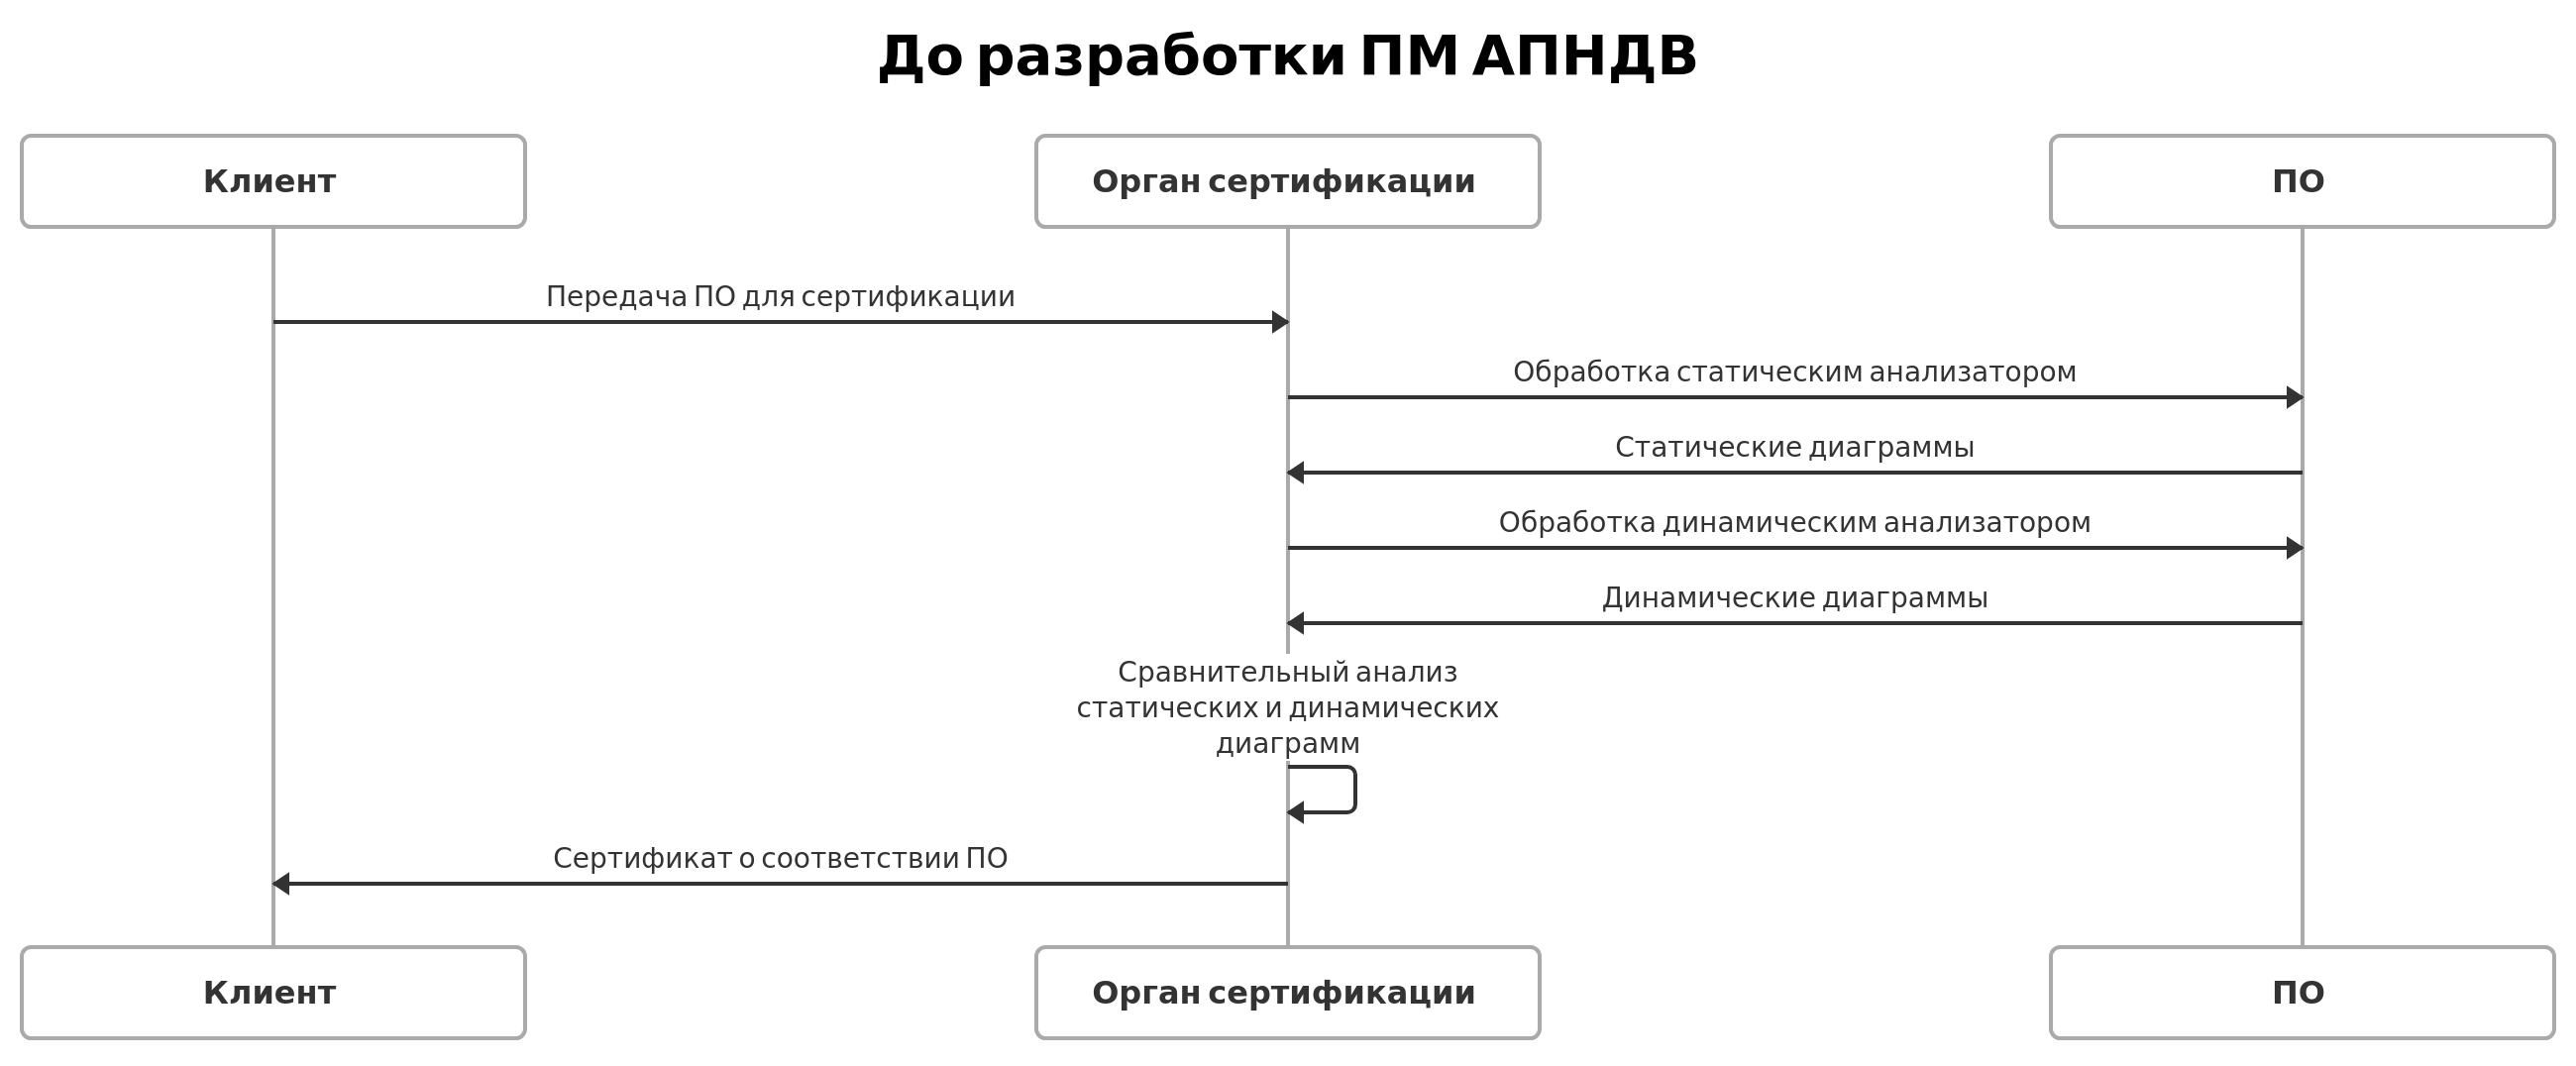
\includegraphics[width=\textwidth,height=\textheight,keepaspectratio]{images/uml_before_cropped.png}
    \end{figure}
    \begin{figure}[!htbp]
    \vspace{-2.6ex} 
        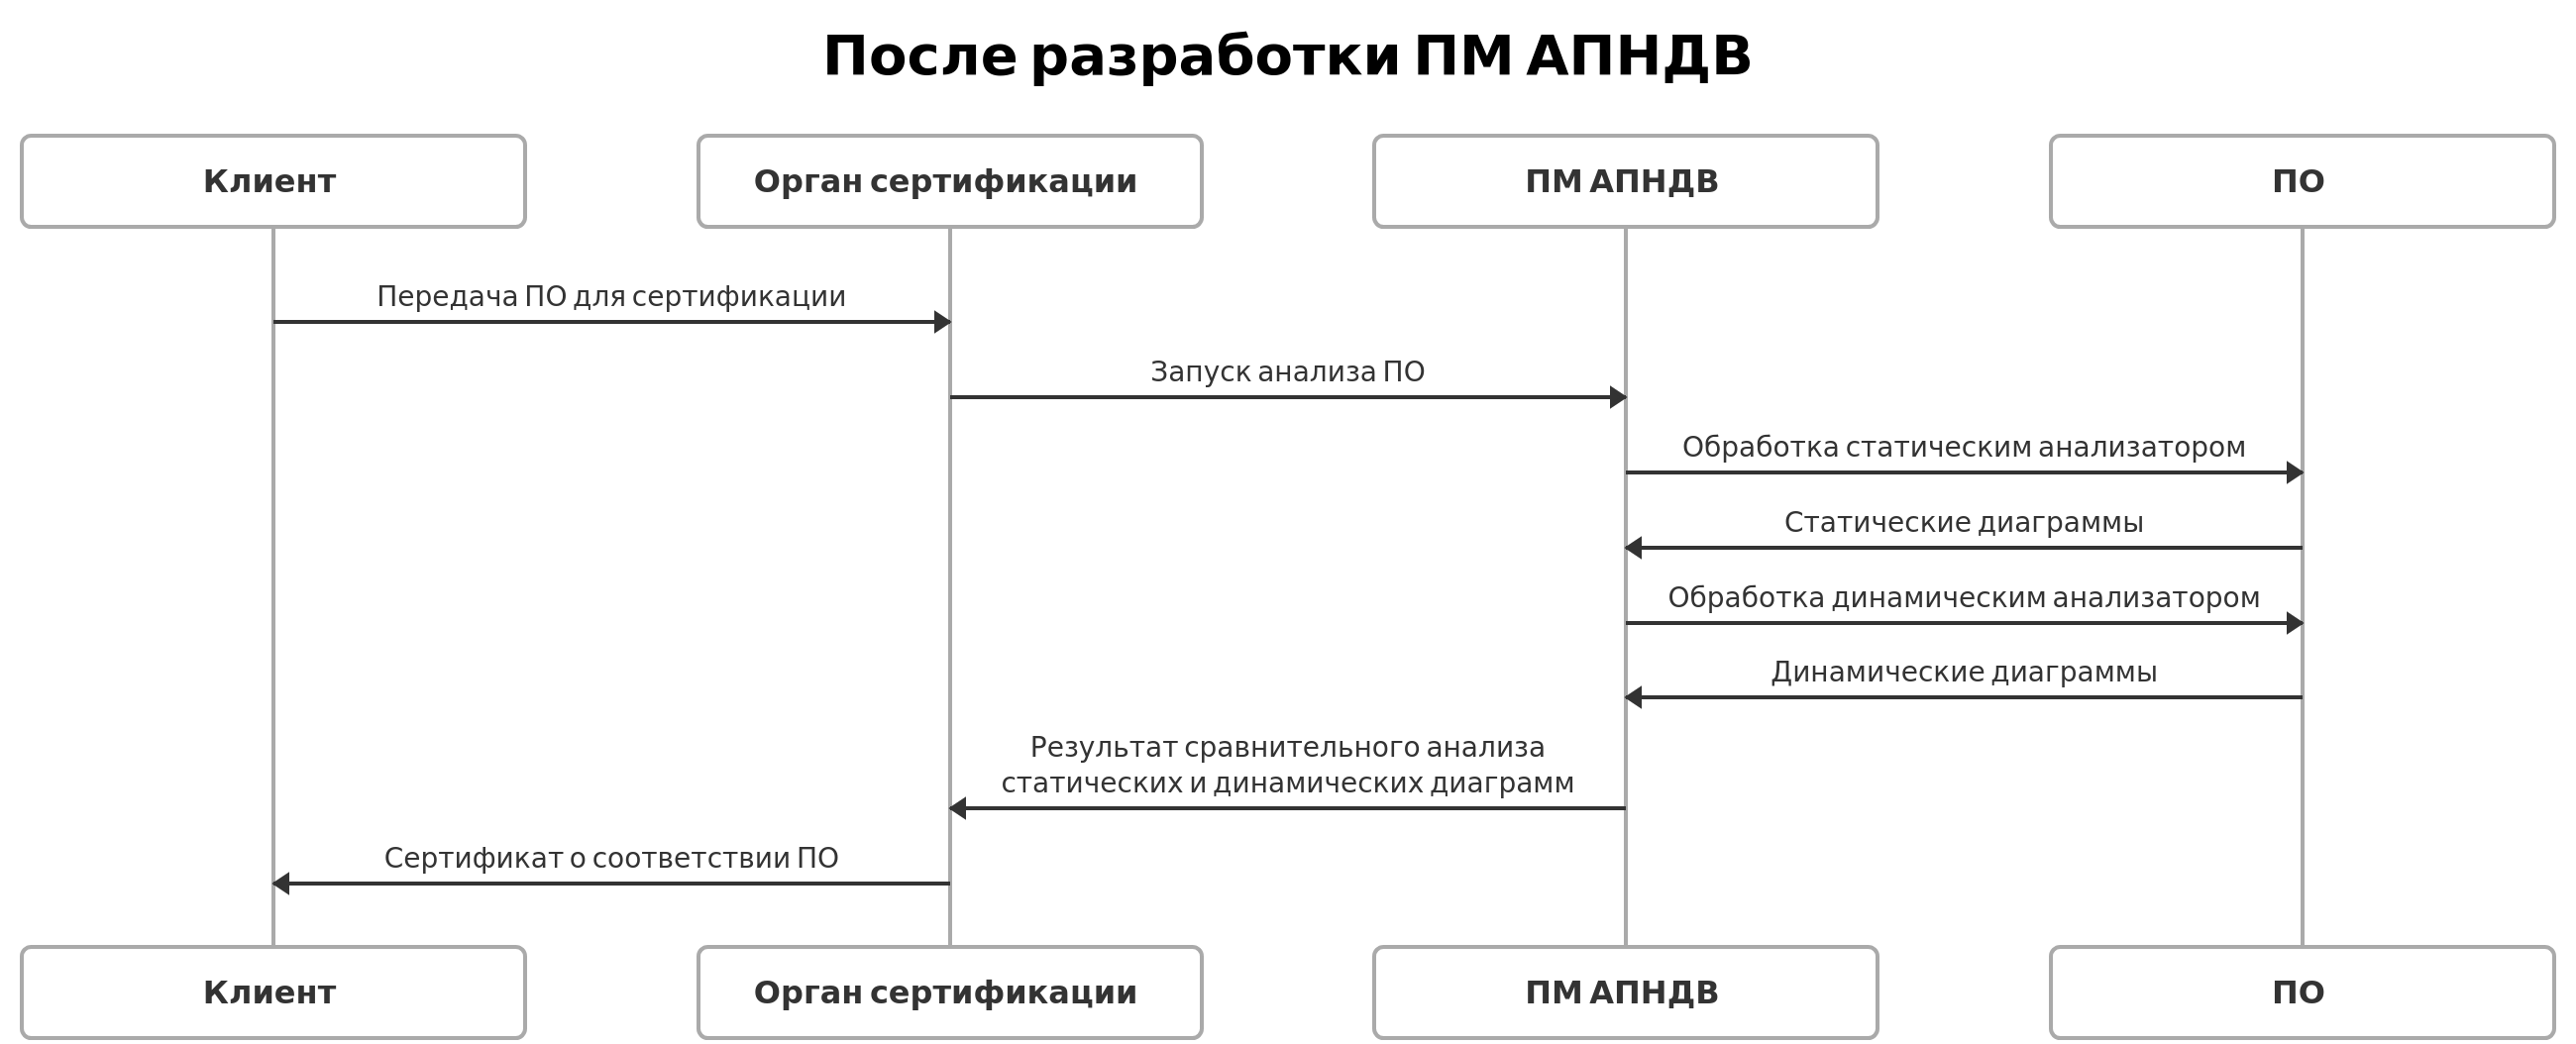
\includegraphics[width=\textwidth,height=\textheight,keepaspectratio]{images/uml_after_cropped.png}
    \end{figure}
%\begin{table}[!htbp]
%    \centering
%    \caption{\label{table:why-am-i-the-best}До и после разработки {\ProgModule}}
%
%    \begin{center}
%        \begin{tabular}{ | c | c | }
%            \hline
%            \makecell{До разработки {\ProgModule}} & \makecell{После разработки {\ProgModule}}\\
%            \hline
%            \makecell{Проведение статического,\\
%                      динамического и сравнительного\\
%                      анализа проходило вручную} & 
%            \makecell{Проведение статического,\\
%                      динамического и сравнительного\\
%                      анализа проходит автоматически}\\
%            \hline
%            \makecell{Для проведения анализов\\
%                      нужно было вручную выбирать\\
%                      исследуемые файлы} & 
%            \makecell{Для проведения анализов,\\
%                      {\ProgModule}\\
%                      делает это автоматически}\\
%            \hline
%            \makecell{Динамический анализ включал\\
%                      в себя только вызовы функций} & 
%            \makecell{Динамический анализ включает\\
%                      в себя информацию о состоянии\\
%                      стека и регистров программы\\
%                      во время конкретного вызова}\\
%            \hline
%        \end{tabular}
%    \end{center}
%
%\end{table}
\end{frame}

\begin{frame}%[plain, noframenumbering, t]
\frametitle{Обзор существующих решений. Статические анализаторы.}

\begin{table}[!htbp]
    {\footnotesize
        \setlength{\tabcolsep}{2pt}
        \begin{longtable}{*{4}{| c}|}
            \hline
            \diagbox[width=4cm]{Свойства}{Название\\программы}                                       &
            \makecell{Microsoft\\Application\\Inspector \autocite{microsoft-application-inspector}} &
            \makecell{SCI\\Tools\\Understand \autocite{sci-tools-understand}}                       &
            \makecell{GNU cflow \autocite{gnu-cflow}} \\
            \hline
            \makecell{Кроссплатформенность}             & \greencell{Да} & \greencell{Да} & \greencell{Да}\\
            \hline
            \makecell{Открытость\\исходного кода}        & \greencell{Да} & \redcell{Нет}   & \greencell{Да}\\
            \hline
            \makecell{Препроцессирование\\кода C/C++}    & \redcell{Нет}   & \greencell{Да} & \greencell{Да}\\
            \hline
            \makecell{Представление\\
                      препроцессорных директив как\\
                      вызов функций}                     & \redcell{Нет}   & \redcell{Нет}   & \greencell{Да}\\
            \hline
            \makecell{Создание графа вызовов}            & \redcell{Нет}   & \greencell{Да} & \greencell{Да} \\
            \hline
            \makecell{Создание обратного\\графа вызовов} & \redcell{Нет}   & \greencell{Да} & \greencell{Да}\\
            \hline
            \makecell{Бесплатность}                      & \greencell{Да} & \redcell{Нет}   & \greencell{Да}\\
            \hline
            \makecell{Графический интерфейс}             & Нет & Есть & Нет \\
            \hline
        \end{longtable}
    }
\end{table}

\vspace{-5ex}
{\scriptsize
\begin{itemize}
    \item \cite{microsoft-application-inspector} \fullcite{microsoft-application-inspector}
    \item \cite{sci-tools-understand} \fullcite{sci-tools-understand}
    \item \cite{gnu-cflow} \fullcite{gnu-cflow}
\end{itemize}
}

\end{frame}

\begin{frame}%[plain, noframenumbering, t]
\frametitle{Обзор существующих решений. Динамические анализаторы.}

\begin{table}[!htbp]
    {\small
        \setlength{\tabcolsep}{2pt}
        \begin{longtable}{*{3}{| c}|}
            \hline
            \diagbox[width=8cm]{Свойства}{Название программы} &
            \makecell{GDB \autocite{gdb}}                     &
            \makecell{QEMU \autocite{qemu}}                   \\
            \hline
            \makecell{Кроссплатформенность}             & \greencell{Да} & \greencell{Да} \\
            \hline
            \makecell{Открытость исходного кода}        & \greencell{Да} & \greencell{Да} \\
            \hline
            \makecell{Возможность анализировать память} & \greencell{Да} & \greencell{Да} \\
            \hline
            \makecell{Возможность программно управлять} & \greencell{Да} & \greencell{Да} \\
            \hline
            \makecell{Возможность создавать 
                      собственные команды}               & \greencell{Да} & \redcell{Нет}   \\
            \hline
            \makecell{Возможность удаленной 
                      отладки}                           & \greencell{Да} & \redcell{Нет}   \\
            \hline
            \makecell{Бесплатность}                      & \greencell{Да} & \greencell{Да} \\
            \hline
            \makecell{Графический интерфейс}             & Есть & Есть \\
            \hline
        \end{longtable}
    }
\end{table}
\vspace{-5ex}
{\scriptsize
\begin{itemize}
    \item \cite{gdb} \fullcite{gdb}
    \item \cite{qemu} \fullcite{qemu}
\end{itemize}
}
\end{frame}

\begin{frame}%[plain, noframenumbering, t]
\frametitle{Выбор языка программирования}

\begin{table}
    {\small
        \setlength{\tabcolsep}{2pt}
        \begin{longtable}{*{5}{| c}|}
            \hline
            \diagbox[width=5cm]{Свойства}{Язык} &
                \makecell{Nim \autocite{nim}} &
                \makecell{Python \autocite{python}} &
                \makecell{Perl \autocite{perl}} &
                \makecell{C/C++ \autocite{cpp}} \\
            \hline
                \makecell{Сверхвысокоуровневость} & 
                \greencell{Да} & 
                \greencell{Да} &
                \greencell{Да} &
                \redcell{Нет} \\
            \hline
                \makecell{Компилируется в\\машинный код} & 
                \greencell{Да} & 
                \redcell{Нет} &
                \redcell{Нет} &
                \greencell{Да} \\
            \hline
                \makecell{Количество функции в\\стандартной библиотеке} & 
                5585 & 
                638 &
                1338 &
                1224 \\
            \hline
                \makecell{Портируемость} & 
                \greencell{Есть} & 
                \greencell{Есть} &
                \greencell{Есть} &
                \yellowcell{\makecell{Есть,\\но неудобная}}\\
            \hline
                \makecell{Встроенная\\генерация документации} & 
                \greencell{Есть} & 
                \greencell{Есть} &
                \greencell{Есть} &
                \redcell{Нет}\\
            \hline
                \makecell{Статическая типизация} & 
                \greencell{Есть} & 
                \redcell{Нет} &
                \redcell{Нет} &
                \greencell{Есть}\\
            \hline
                \makecell{Автоматическое\\управление памятью} & 
                \greencell{Есть} & 
                \greencell{Есть} &
                \greencell{Есть} &
                \greencell{Есть} \\
            \hline
                \makecell{Обобщенное программирование} & 
                \greencell{Есть} & 
                \greencell{Есть} &
                \greencell{Есть} &
                \greencell{Есть} \\
            \hline
                \makecell{Метапрограммирование} & 
                \greencell{Есть} & 
                \greencell{Есть} &
                \greencell{Есть} &
                \greencell{Есть} \\
            \hline
                \makecell{Опыт использования} & 
                \greencell{Есть} & 
                \greencell{Есть} &
                \redcell{Нет} &
                \greencell{Есть} \\
            \hline
        \end{longtable}
    }
\end{table}
\vspace{-5ex}
{\scriptsize
\begin{itemize}
    \item \cite{nim} \fullcite{nim}
    \item \cite{python} \fullcite{python}
    \item \cite{perl} \fullcite{perl}
\end{itemize}
}

\end{frame}

\begin{frame}%[plain, noframenumbering, t]
\frametitle{Выбор среды разработки}

\begin{table}[!htbp]
    {\small
        \setlength{\tabcolsep}{2pt}
        \begin{longtable}{*{6}{| c}|}
            \hline
            \diagbox[width=4cm]{Свойства}{IDE/Редактор} &
                \makecell{Aporia \autocite{aporia-ide}} &
                \makecell{Atom \autocite{atom-ide}} &
                \makecell{Sublime\\Text \autocite{sublime-ide}} &
                \makecell{Visual\\Studio\\Code \autocite{vs-code-ide}} &
                \makecell{Vim \autocite{vim-ide}} \\
            \hline
                \makecell{Поддержка плагинов} & 
                \redcell{Нет} &
                \greencell{Да} & 
                \greencell{Да} &
                \greencell{Да} &
                \greencell{Да} \\
            \hline
                \makecell{Требователен к ресурсам} & 
                \greencell{Нет} & 
                \redcell{Да} & 
                \greencell{Нет} & 
                \redcell{Да} & 
                \greencell{Нет} \\ 
            \hline
                \makecell{Имеет продвинутую систему\\редактирования текста} & 
                \redcell{Нет} &
                \redcell{Нет} &
                \redcell{Нет} &
                \redcell{Нет} &
                \greencell{Да} \\
            \hline
                \makecell{Кроссплатформенность} & 
                \greencell{Есть} & 
                \greencell{Есть} &
                \greencell{Есть} &
                \greencell{Есть} &
                \greencell{Есть} \\
            \hline
                \makecell{Может работать\\без GUI} & 
                \redcell{Нет} &
                \redcell{Нет} &
                \redcell{Нет} &
                \redcell{Нет} &
                \greencell{Да} \\
            \hline
                \makecell{Восстановление после сбоев} & 
                \redcell{Нет} & 
                \greencell{Есть} &
                \greencell{Есть} &
                \greencell{Есть} &
                \greencell{Есть} \\
            \hline
                \makecell{Возможность выделять\\ключевые слова с помощью\\регулярных выражений} & 
                \redcell{Нет} & 
                \greencell{Есть} &
                \greencell{Есть} &
                \greencell{Есть} &
                \greencell{Есть} \\
            \hline
                \makecell{Опыт использования} & 
                \redcell{Нет} &
                \redcell{Нет} &
                \greencell{Есть} &
                \greencell{Есть} &
                \greencell{Есть} \\
            \hline
        \end{longtable}
    }
\end{table}

\vspace{-5ex}
{\scriptsize
\begin{itemize}
    \item \cite{aporia-ide} \fullcite{aporia-ide}
    \item \cite{atom-ide} \fullcite{atom-ide}
    \item \cite{sublime-ide} \fullcite{sublime-ide}
    \item \cite{vs-code-ide} \fullcite{vs-code-ide}
    \item \cite{vim-ide} \fullcite{vim-ide}
\end{itemize}
}
\end{frame}

\begin{frame}%[plain, noframenumbering, t]
\frametitle{Схема данных {\ProgModule}}
    \begin{figure}[!htbp]
        % !TEX encoding = UTF-8 Unicode
% Úτƒ-8 encoded
% http://www.linux.org.ru/forum/general/10357036
\tikzset{
    line/.style={draw, -latex'},
    every join/.style={line},
    u/.style={anchor=south},
    r/.style={anchor=west},
    fxd/.style={text width = 6em},
    it/.style={font={\small\itshape}},
    bf/.style={font={\small\bfseries}}

}
\tikzstyle{base} =
    [
        draw,
        on chain,
        on grid,
        align=center,
        minimum height=4ex,
        minimum width = 5ex,
        node distance = 6mm and 60mm,
        text badly centered,
        text width=5cm
    ]
\tikzstyle{coord} =
    [
        coordinate,
        on chain,
        on grid
    ]
\tikzstyle{cloud} =
    [
        base,
        ellipse,
        node distance = 3cm,
        minimum height = 2em
    ]
\tikzstyle{decision} =
    [
        base,
        diamond,
        aspect=2,
        node distance = 2cm,
        inner sep = 0pt
    ]
\tikzstyle{block} =
    [
        rectangle,
        base,
        rounded corners,
        minimum height = 2em
    ]
\tikzstyle{print_block} =
    [
        base,
        tape,
        tape bend top=none,
    ]
\tikzstyle{io} =
    [
        base,
        trapezium,
        trapezium left angle = 70,
        trapezium right angle = 110,
    ]
\tikzstyle{prompt} =
    [
        base,
        trapezium,
        trapezium left angle = 90,
        trapezium right angle = 80,
        shape border rotate = 90
    ]
\tikzstyle{disk file} =
    [
        base,
        cylinder,
        aspect=0.2,
    ]
\tikzstyle{process} =
    [
        rectangle,
        base,
    ]
\makeatletter
\pgfkeys{/pgf/.cd,
    subrtshape w/.initial=2mm,
    cycleshape w/.initial=2mm
}
\pgfdeclareshape{subrtshape}{
    \inheritsavedanchors[from=rectangle]
    \inheritanchorborder[from=rectangle]
    \inheritanchor[from=rectangle]{north}
    \inheritanchor[from=rectangle]{center}
    \inheritanchor[from=rectangle]{west}
    \inheritanchor[from=rectangle]{east}
    \inheritanchor[from=rectangle]{mid}
    \inheritanchor[from=rectangle]{base}
    \inheritanchor[from=rectangle]{south}
    \backgroundpath{
        \southwest \pgf@xa=\pgf@x \pgf@ya=\pgf@y
        \northeast \pgf@xb=\pgf@x \pgf@yb=\pgf@y
        \pgfmathsetlength\pgfutil@tempdima{\pgfkeysvalueof{/pgf/subrtshape w}}
        \def\ppd@offset{\pgfpoint{\pgfutil@tempdima}{0ex}}
        \def\ppd@offsetm{\pgfpoint{-\pgfutil@tempdima}{0ex}}
        \pgfpathmoveto{\pgfqpoint{\pgf@xa}{\pgf@ya}}
        \pgfpathlineto{\pgfqpoint{\pgf@xb}{\pgf@ya}}
        \pgfpathlineto{\pgfqpoint{\pgf@xb}{\pgf@yb}}
        \pgfpathlineto{\pgfqpoint{\pgf@xa}{\pgf@yb}}
        \pgfpathclose
        \pgfpathmoveto{\pgfpointadd{\pgfpoint{\pgf@xa}{\pgf@yb}}{\ppd@offsetm}}
        \pgfpathlineto{\pgfpointadd{\pgfpoint{\pgf@xa}{\pgf@ya}}{\ppd@offsetm}}
        \pgfpathlineto{\pgfpointadd{\pgfpoint{\pgf@xb}{\pgf@ya}}{\ppd@offset}}
        \pgfpathlineto{\pgfpointadd{\pgfpoint{\pgf@xb}{\pgf@yb}}{\ppd@offset}}
        \pgfpathclose
    }
}
\pgfdeclareshape{cyclebegshape}{
    \inheritsavedanchors[from=rectangle]
    \inheritanchorborder[from=rectangle]
    \inheritanchor[from=rectangle]{north}
    \inheritanchor[from=rectangle]{center}
    \inheritanchor[from=rectangle]{west}
    \inheritanchor[from=rectangle]{east}
    \inheritanchor[from=rectangle]{mid}
    \inheritanchor[from=rectangle]{base}
    \inheritanchor[from=rectangle]{south}
    \backgroundpath{
        \southwest \pgf@xa=\pgf@x \pgf@ya=\pgf@y
        \northeast \pgf@xb=\pgf@x \pgf@yb=\pgf@y
        \pgfmathsetlength\pgfutil@tempdima{\pgfkeysvalueof{/pgf/cycleshape w}}
        \pgfpathmoveto{\pgfqpoint{\pgf@xa}{\pgf@ya}}
\pgfpathlineto{\pgfpointadd{\pgfpoint{\pgf@xa}{\pgf@yb}}{\pgfpoint{0ex}{-\pgfutil@tempdima}}}
\pgfpathlineto{\pgfpointadd{\pgfpoint{\pgf@xa}{\pgf@yb}}{\pgfpoint{\pgfutil@tempdima}{0ex}}}
\pgfpathlineto{\pgfpointadd{\pgfpoint{\pgf@xb}{\pgf@yb}}{\pgfpoint{-\pgfutil@tempdima}{0ex}}}
\pgfpathlineto{\pgfpointadd{\pgfpoint{\pgf@xb}{\pgf@yb}}{\pgfpoint{0ex}{-\pgfutil@tempdima}}}
\pgfpathlineto{\pgfqpoint{\pgf@xb}{\pgf@ya}}
        \pgfpathclose
    }
}
\pgfdeclareshape{cycleendshape}{
    \inheritsavedanchors[from=rectangle]
    \inheritanchorborder[from=rectangle]
    \inheritanchor[from=rectangle]{north}
    \inheritanchor[from=rectangle]{center}
    \inheritanchor[from=rectangle]{west}
    \inheritanchor[from=rectangle]{east}
    \inheritanchor[from=rectangle]{mid}
    \inheritanchor[from=rectangle]{base}
    \inheritanchor[from=rectangle]{south}
    \backgroundpath{
        \southwest \pgf@xa=\pgf@x \pgf@ya=\pgf@y
        \northeast \pgf@xb=\pgf@x \pgf@yb=\pgf@y
        \pgfmathsetlength\pgfutil@tempdima{\pgfkeysvalueof{/pgf/cycleshape w}}
        \pgfpathmoveto{\pgfqpoint{\pgf@xb}{\pgf@yb}}
\pgfpathlineto{\pgfpointadd{\pgfpoint{\pgf@xb}{\pgf@ya}}{\pgfpoint{0ex}{\pgfutil@tempdima}}}
\pgfpathlineto{\pgfpointadd{\pgfpoint{\pgf@xb}{\pgf@ya}}{\pgfpoint{-\pgfutil@tempdima}{0ex}}}
\pgfpathlineto{\pgfpointadd{\pgfpoint{\pgf@xa}{\pgf@ya}}{\pgfpoint{\pgfutil@tempdima}{0ex}}}
\pgfpathlineto{\pgfpointadd{\pgfpoint{\pgf@xa}{\pgf@ya}}{\pgfpoint{0ex}{\pgfutil@tempdima}}}
\pgfpathlineto{\pgfqpoint{\pgf@xa}{\pgf@yb}}
        \pgfpathclose
    }
}
\makeatother
\tikzstyle{subroutine} =
    [
        base,
        subrtshape,
    ]
\tikzstyle{cyclebegin} =
    [
        base,
        cyclebegshape,
    ]
\tikzstyle{cycleend} =
    [
        base,
        cycleendshape,
    ]
\tikzstyle{connector} =
    [
        base,
        circle,
    ]
\begin{tikzpicture}[%
    start chain=going below,    % General flow is top-to-bottom
    node distance=6mm and 30mm, % Global setup of box spacing
    scale=0.7, 
    every node/.style={scale=0.72}
    ] 
        \node [prompt   ] (makefile path)   [left  = 2cm ]                               {\small Путь до папки с Makefile};
        \node [process  ] (builder)         [below = 0.7cm of makefile path]             {\small Сборщик};
        \node [disk file] (makefile)        [yshift=0.5cm, left  = 5cm of makefile path] {\small Makefile};
        \node [prompt   ] (executable)      [right = 10cm of makefile path]              {\small Путь до исполняемого файла};
        \node [process  ] (breakpointer)                                                 {\small Модуль бинарного анализа};
        \node [disk file] (modified exe)    [xshift=3.5cm, below = 1cm of breakpointer]  {\small Модифицированный исполняемый файл};
        \node [disk file] (build log)       [xshift=3.5cm, below = 1cm of builder]       {\small Файл с информацией о сборке};
        \node [disk file] (call map)        [left = 8.25cm of build log]                 {\small Файл с информацией о линковке};
        \node [process  ] (static analyzer) [below = 1.25cm of build log]                {\small Модуль статического анализа};
        \node [disk file] (sources)         [left = 4.15cm of build log]                 {\small Файлы с исходным кодом};
        \node [disk file] (gdb script)      [left = 5cm of modified exe]                 {\small Скрипт для GDB};
        \node [process  ] (gdb manager)     [below = 2.25cm of breakpointer]             {\small Модуль управления отладчиком};
        \node [disk file] (dyn result)      [below = 1.25cm of gdb manager]              {\small Результаты динамического анализа};
        \node [process  ] (dyn parser)      [below = 1.25cm of dyn result]               {\small Модуль преобразования результатов динамического анализа};
        \node [disk file] (dyn json)        [below = 1.25cm of dyn parser]               {\small Преобразованные результаты динамического анализа};
        \node [disk file] (stat result)     [below = 1.25cm of static analyzer]          {\small Результаты статического анализа};
        \node [process  ] (stat parser)     [below = 1.25cm of stat result]              {\small Модуль преобразования результатов статического анализа};
        \node [disk file] (stat json)       [below = 1.25cm of stat parser]              {\small Преобразованные результаты статического анализа};
        \node [process  ] (aggregator)      [below = 1.25cm of stat json]                {\small Модуль агрегирования результатов линковки и статического анализа};
        \node [disk file] (aggregator file) [below = 1.25cm of aggregator]               {\small Агрегированные результаты линковки и статического анализа};
        \node [process  ] (comparer)                                                     {\small Модуль сравнительного анализа};
        \node [disk file] (summary)                                                      {\small Результаты сравнительного анализа};
        \node [disk file] (file executable) [left = 4.5cm of executable]                 {\small Исполняемый\\файл};

        \draw [-] (makefile path)      -- (builder);
        \draw [-] (makefile)           -- +(0,-0.95) -| (builder);
        \draw [line] (builder)         -| (call map);
        \draw [line] (builder)         -| (build log);

        \draw [line] (executable)      -- (breakpointer);
        \draw [line] (file executable) -- +(0,-0.7) -| (breakpointer);
        \draw [line] (breakpointer)    -| (modified exe);
        \draw [line] (breakpointer)    -| (gdb script);

        \draw [line] (modified exe)    |- (gdb manager);
        \draw [line] (gdb script)      |- (gdb manager);
        \draw [line] (gdb manager)     -- (dyn result);
        \draw [line] (dyn result)      -- (dyn parser);
        \draw [line] (dyn parser)      -- (dyn json);


        \draw [line] (build log)       -- (static analyzer);
        \draw [line] (static analyzer) -- (stat result);
        \draw [line] (stat result)     -- (stat parser);
        \draw [line] (stat parser)     -- (stat json);
        \draw [line] (call map)        |- (aggregator);
        \draw [line] (stat json)       -- (aggregator);
        \draw [line] (aggregator)      -- (aggregator file);
        \draw [line] (sources)         |- (static analyzer);

        \draw [line] (aggregator file) -- (comparer);
        \draw [line] (dyn json)        |- (comparer);
        \draw [line] (comparer)        -- (summary);

\end{tikzpicture}

    \end{figure}
\end{frame}

\begin{frame}%[plain, noframenumbering, t]
\frametitle{Схема алгоритма {\ProgModule}}

    \Put(149,-414){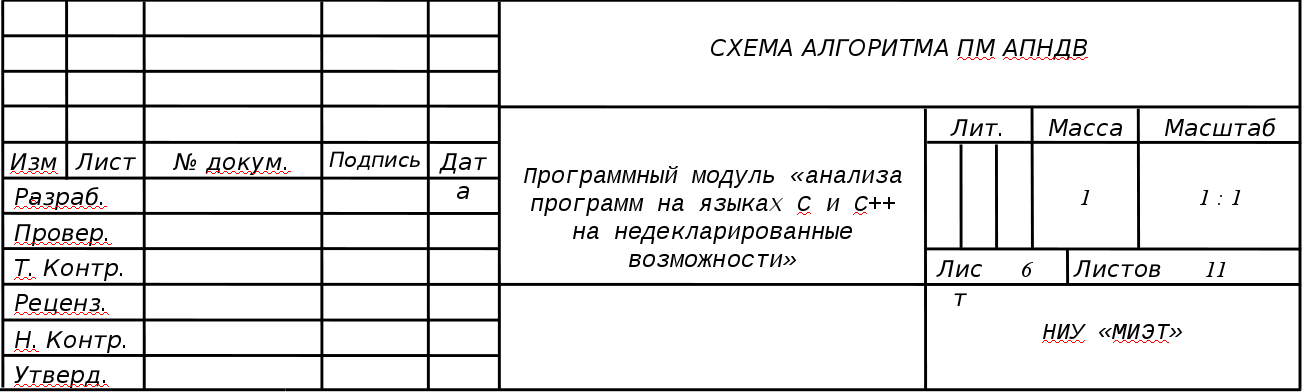
\includegraphics[height=2cm]{Presentation/images/algo_gost.png}}
    %\begin{figure}[!htbp]
    %    \begin{adjustbox}{max totalsize={1.0\textwidth}{0.8\textheight},left}
    %        \includegraphics{}
    %    \end{adjustbox}
    %\end{figure}

    \begin{figure}[!htbp]
        \vspace{-9ex} 
        \hspace{-13cm} 
        \begin{adjustbox}{max totalsize={1.6\textwidth}{1.6\textheight},left}
            % !TEX encoding = UTF-8 Unicode
% Úτƒ-8 encoded
% http://www.linux.org.ru/forum/general/10357036
\tikzset{
    line/.style={draw, -latex'},
    every join/.style={line},
    u/.style={anchor=south},
    r/.style={anchor=west},
    fxd/.style={text width = 6em},
    it/.style={font={\small\itshape}},
    bf/.style={font={\small\bfseries}},
}
\tikzstyle{base_long} =
    [
        draw,
        on chain,
        on grid,
        align=center,
        minimum height=4ex,
        minimum width = 10ex,
        node distance = 6mm and 60mm,
        text badly centered,
    ]
\tikzstyle{base} =
    [
        draw,
        on chain,
        on grid,
        align=center,
        minimum height=4ex,
        minimum width = 10ex,
        node distance = 6mm and 60mm,
        text badly centered,
        text width=5cm
    ]
\tikzstyle{coord} =
    [
        coordinate,
        on chain,
        on grid
    ]
\tikzstyle{cloud} =
    [
        base,
        ellipse,
        node distance = 3cm,
        minimum height = 2em,
        text width=2cm
    ]
\tikzstyle{decision} =
    [
        base,
        diamond,
        aspect=2,
        node distance = 2cm,
        inner sep = 0pt
    ]
\tikzstyle{block} =
    [
        rectangle,
        base,
        rounded corners,
        minimum height = 2em
    ]
\tikzstyle{print_block} =
    [
        base,
        tape,
        tape bend top=none,
    ]
\tikzstyle{io} =
    [
        base,
        trapezium,
        trapezium left angle = 70,
        trapezium right angle = 110,
    ]
\tikzstyle{prompt} =
    [
        base,
        trapezium,
        trapezium left angle = 90,
        trapezium right angle = 80,
        shape border rotate = 90
    ]
\tikzstyle{disk file} =
    [
        base,
        cylinder,
        aspect=0.2,
    ]
\tikzstyle{process} =
    [
        rectangle,
        base,
    ]
\makeatletter
\pgfkeys{/pgf/.cd,
    subrtshape w/.initial=2mm,
    cycleshape w/.initial=2mm
}
\pgfdeclareshape{parallelshape}{
    \inheritsavedanchors[from=rectangle]
    \inheritanchorborder[from=rectangle]
    \inheritanchor[from=rectangle]{north}
    \inheritanchor[from=rectangle]{center}
    \inheritanchor[from=rectangle]{west}
    \inheritanchor[from=rectangle]{east}
    \inheritanchor[from=rectangle]{mid}
    \inheritanchor[from=rectangle]{base}
    \inheritanchor[from=rectangle]{south}
    \backgroundpath{
        \southwest \pgf@xa=\pgf@x \pgf@ya=\pgf@y
        \northeast \pgf@xb=\pgf@x \pgf@yb=\pgf@y
        \def\ppd@offset{\pgfpoint{\pgfutil@tempdima}{0ex}}
        \def\ppd@offsetm{\pgfpoint{-\pgfutil@tempdima}{0ex}}
        \pgfpathmoveto{\pgfqpoint{\pgf@xa}{\pgf@ya}}
            \pgfpathlineto{\pgfqpoint{\pgf@xb}{\pgf@ya}}
        \pgfpathclose
        \pgfpathmoveto{\pgfqpoint{\pgf@xb}{\pgf@yb}}
            \pgfpathlineto{\pgfqpoint{\pgf@xa}{\pgf@yb}}
        \pgfpathclose
    }
}
\pgfdeclareshape{subrtshape}{
    \inheritsavedanchors[from=rectangle]
    \inheritanchorborder[from=rectangle]
    \inheritanchor[from=rectangle]{north}
    \inheritanchor[from=rectangle]{center}
    \inheritanchor[from=rectangle]{west}
    \inheritanchor[from=rectangle]{east}
    \inheritanchor[from=rectangle]{mid}
    \inheritanchor[from=rectangle]{base}
    \inheritanchor[from=rectangle]{south}
    \backgroundpath{
        \southwest \pgf@xa=\pgf@x \pgf@ya=\pgf@y
        \northeast \pgf@xb=\pgf@x \pgf@yb=\pgf@y
        \pgfmathsetlength\pgfutil@tempdima{\pgfkeysvalueof{/pgf/subrtshape w}}
        \def\ppd@offset{\pgfpoint{\pgfutil@tempdima}{0ex}}
        \def\ppd@offsetm{\pgfpoint{-\pgfutil@tempdima}{0ex}}
        \pgfpathmoveto{\pgfqpoint{\pgf@xa}{\pgf@ya}}
        \pgfpathlineto{\pgfqpoint{\pgf@xb}{\pgf@ya}}
        \pgfpathlineto{\pgfqpoint{\pgf@xb}{\pgf@yb}}
        \pgfpathlineto{\pgfqpoint{\pgf@xa}{\pgf@yb}}
        \pgfpathclose
        \pgfpathmoveto{\pgfpointadd{\pgfpoint{\pgf@xa}{\pgf@yb}}{\ppd@offsetm}}
        \pgfpathlineto{\pgfpointadd{\pgfpoint{\pgf@xa}{\pgf@ya}}{\ppd@offsetm}}
        \pgfpathlineto{\pgfpointadd{\pgfpoint{\pgf@xb}{\pgf@ya}}{\ppd@offset}}
        \pgfpathlineto{\pgfpointadd{\pgfpoint{\pgf@xb}{\pgf@yb}}{\ppd@offset}}
        \pgfpathclose
    }
}
\pgfdeclareshape{cyclebegshape}{
    \inheritsavedanchors[from=rectangle]
    \inheritanchorborder[from=rectangle]
    \inheritanchor[from=rectangle]{north}
    \inheritanchor[from=rectangle]{center}
    \inheritanchor[from=rectangle]{west}
    \inheritanchor[from=rectangle]{east}
    \inheritanchor[from=rectangle]{mid}
    \inheritanchor[from=rectangle]{base}
    \inheritanchor[from=rectangle]{south}
    \backgroundpath{
        \southwest \pgf@xa=\pgf@x \pgf@ya=\pgf@y
        \northeast \pgf@xb=\pgf@x \pgf@yb=\pgf@y
        \pgfmathsetlength\pgfutil@tempdima{\pgfkeysvalueof{/pgf/cycleshape w}}
        \pgfpathmoveto{\pgfqpoint{\pgf@xa}{\pgf@ya}}
\pgfpathlineto{\pgfpointadd{\pgfpoint{\pgf@xa}{\pgf@yb}}{\pgfpoint{0ex}{-\pgfutil@tempdima}}}
\pgfpathlineto{\pgfpointadd{\pgfpoint{\pgf@xa}{\pgf@yb}}{\pgfpoint{\pgfutil@tempdima}{0ex}}}
\pgfpathlineto{\pgfpointadd{\pgfpoint{\pgf@xb}{\pgf@yb}}{\pgfpoint{-\pgfutil@tempdima}{0ex}}}
\pgfpathlineto{\pgfpointadd{\pgfpoint{\pgf@xb}{\pgf@yb}}{\pgfpoint{0ex}{-\pgfutil@tempdima}}}
\pgfpathlineto{\pgfqpoint{\pgf@xb}{\pgf@ya}}
        \pgfpathclose
    }
}
\pgfdeclareshape{cycleendshape}{
    \inheritsavedanchors[from=rectangle]
    \inheritanchorborder[from=rectangle]
    \inheritanchor[from=rectangle]{north}
    \inheritanchor[from=rectangle]{center}
    \inheritanchor[from=rectangle]{west}
    \inheritanchor[from=rectangle]{east}
    \inheritanchor[from=rectangle]{mid}
    \inheritanchor[from=rectangle]{base}
    \inheritanchor[from=rectangle]{south}
    \backgroundpath{
        \southwest \pgf@xa=\pgf@x \pgf@ya=\pgf@y
        \northeast \pgf@xb=\pgf@x \pgf@yb=\pgf@y
        \pgfmathsetlength\pgfutil@tempdima{\pgfkeysvalueof{/pgf/cycleshape w}}
        \pgfpathmoveto{\pgfqpoint{\pgf@xb}{\pgf@yb}}
\pgfpathlineto{\pgfpointadd{\pgfpoint{\pgf@xb}{\pgf@ya}}{\pgfpoint{0ex}{\pgfutil@tempdima}}}
\pgfpathlineto{\pgfpointadd{\pgfpoint{\pgf@xb}{\pgf@ya}}{\pgfpoint{-\pgfutil@tempdima}{0ex}}}
\pgfpathlineto{\pgfpointadd{\pgfpoint{\pgf@xa}{\pgf@ya}}{\pgfpoint{\pgfutil@tempdima}{0ex}}}
\pgfpathlineto{\pgfpointadd{\pgfpoint{\pgf@xa}{\pgf@ya}}{\pgfpoint{0ex}{\pgfutil@tempdima}}}
\pgfpathlineto{\pgfqpoint{\pgf@xa}{\pgf@yb}}
        \pgfpathclose
    }
}
\makeatother
\tikzstyle{subroutine} =
    [
        base,
        subrtshape,
    ]
\tikzstyle{cyclebegin} =
    [
        base,
        cyclebegshape,
    ]
\tikzstyle{cycleend} =
    [
        base,
        cycleendshape,
    ]
\tikzstyle{connector} =
    [
        base,
        circle,
    ]

\tikzstyle{parallel} =
    [
        base_long,
        parallelshape,
    ]
\begin{tikzpicture}[%
    start chain=going below,    % General flow is top-to-bottom
    node distance=6mm and 30mm, % Global setup of box spacing
    ] 
        \node [cloud    ] (makefile)        [left  = 4cm ]                   {\small Начало};
        \node [process  ] (builder)         [below = 1cm of makefile]        {\small Сборщик};
        \node [parallel ] (parallel)        [below of = builder, yscale=0.3] {\rptf[105]{\ }};
        \node [process  ] (breakpointer)    [below right = 5cm of builder]   {\small Бинарный анализ};
        \node [process  ] (static analyzer) [below left = 5cm of builder]    {\small Статический анализ};
        \node [process  ] (stat parser)     [below = 2cm of static analyzer] {\small Преобразование результатов статического анализа};
        \node [process  ] (aggregator)      [below = 2cm of stat parser]     {\small Агрегирование результатов линковки и статического анализа};
        \node [process  ] (gdb manager)     [below = 2cm of breakpointer]    {\small Динамический анализ};
        \node [process  ] (dyn parser)      [below = 2cm of gdb manager]     {\small Преобразование результатов динамического анализа};
        \node [cloud    ] (end)             [below = 15cm of makefile]       {\small Конец};
        \node [process  ] (comparer)        [above = 2cm of end]             {\small Сравнительный анализ};
        \node [parallel ] (parallel aggr)   [above = 2cm of comparer, yscale=0.3] {\rpts[105]{\ }};

        \draw [line] (makefile) -- (builder);
        \draw [-] (builder)     -- (parallel);

        \draw [-] (parallel)  -- +(-3.55,-0.095) -- +(-3.55,-1.2) -- (static analyzer);
        \draw [-] (parallel)  -- +(+3.55,-0.095) -- +(+3.55,-1.2) -- (breakpointer);

        \draw [line] (static analyzer) -- (stat parser);
        \draw [line] (stat parser)     -- (aggregator);

        \draw [line] (breakpointer)    -- (gdb manager);
        \draw [line] (gdb manager)     -- (dyn parser);

        \draw [-] (aggregator) -- +(+0,-1.05) -- +(+0,-2.37) -- (parallel aggr);
        \draw [-] (dyn parser) -- +(-0,-1.09) -- +(-0,-2.37) -- (parallel aggr);
        \draw [-] (parallel aggr) -- (comparer);
        \draw [line] (comparer)   -- (end);

\end{tikzpicture}

        \end{adjustbox}
        %\caption{Схема алгоритма {\ProgModule}\label{fig:algorithm}}
    \end{figure}
\end{frame}

\begin{frame}%[plain, noframenumbering, t]
\frametitle{Пользовательский интерфейс {\ProgModule}}
    Пользователь может управлять {\ProgModule} как с помощью
    консольного интерфейса, так и графического.
    \begin{figure}[!htbp]
        \begin{adjustbox}{max totalsize={0.8\textwidth}{0.8\textheight}}
            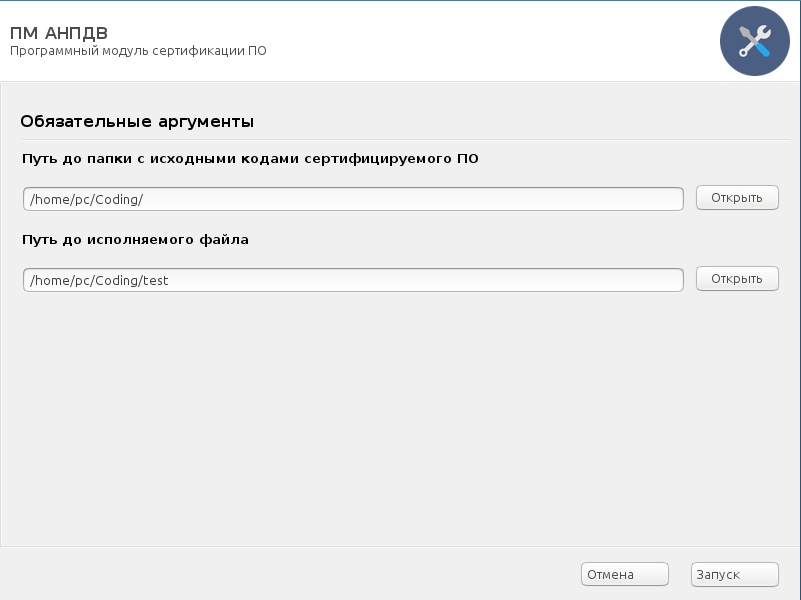
\includegraphics[trim={0.2em 0.2ex 0.2ex 0.2ex},clip,width=\linewidth]{images/apndv-gui.png}
        \end{adjustbox}
        %\caption{Схема алгоритма {\ProgModule}\label{fig:algorithm}}
    \end{figure}

\end{frame}

\begin{frame}%[plain, noframenumbering, t]
\frametitle{Отладка и тестирование {\ProgModule}}
    В процессе разработки {\ProgModule} было написано 43 модульных теста, рассматривающих
    различные сценарии использования элементов {\ProgModule}. {\ProgModule} отлаживался
    с помощью отладчика GDB.
    
    \vspace{3ex}
    \begin{figure}[!htbp]
        \begin{adjustbox}{max totalsize={1.2\textwidth}{1.2\textheight}}
            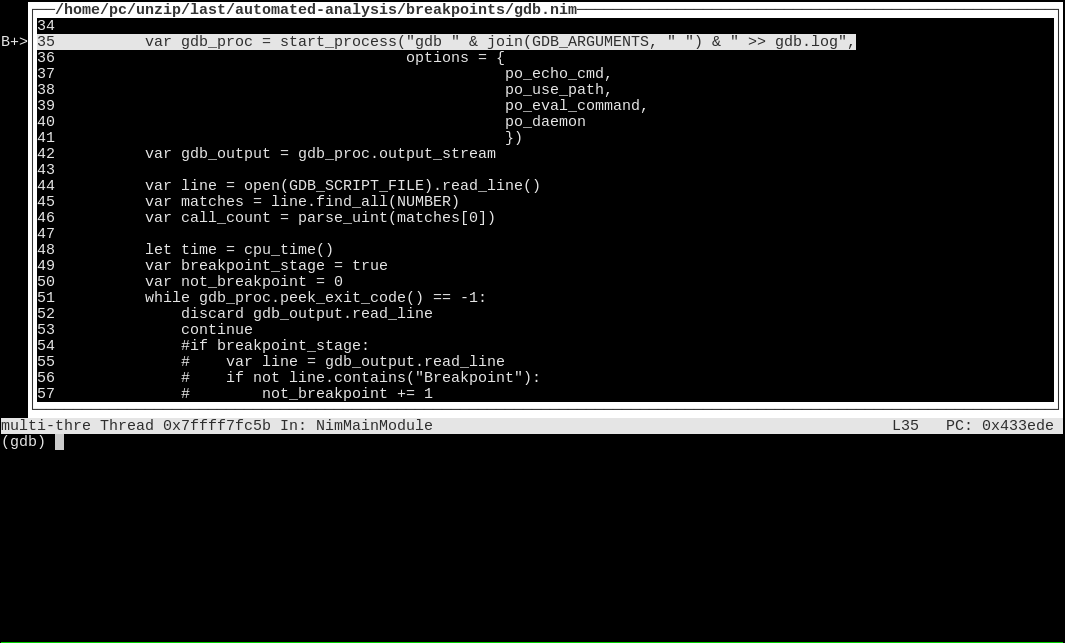
\includegraphics[trim={0 24ex 0 0 0},clip,width=\linewidth]{images/running-gdb.png}
        \end{adjustbox}
        %\caption{Схема алгоритма {\ProgModule}\label{fig:algorithm}}
    \end{figure}

\end{frame}

\begin{frame}%[plain, noframenumbering, t]
\frametitle{Апробация}
    \begin{itemize}
        \item Уманский А.А. Разработка coreutils на языке Forth для встраиваемых систем.
            <<Актуальные проблемы информатизации в цифровой экономике и научных исследованиях>>
            Международная научно-практическая конференция 2019.
        \item Внедрение {\ProgModule} готовится в ООО Фирма <<Анкад>>.
    \end{itemize}
    \begin{figure}[!htbp]
        \begin{adjustbox}{max totalsize={0.6\textwidth}{0.6\textheight}}
            \includegraphics[trim={0 4ex 0 0 0},clip,width=\linewidth]{Presentation/images/conference.jpg}
        \end{adjustbox}
        %\caption{Схема алгоритма {\ProgModule}\label{fig:algorithm}}
    \end{figure}
\end{frame}

\begin{frame}%[plain, noframenumbering, t]
\frametitle{Результаты работы}
    \begin{itemize}
        \item исследована предметная область;
        \item проведен сравнительный анализ существующих программных решений;
        \item выборан язык и среда разработки;
        \item разработана схема данных {\ProgModule};
        \item разработана схема алгоритма {\ProgModule};
        \item программно реализован {\ProgModule};
        \item проведена отладка и тестирование {\ProgModule};
        \item разработано руководство оператора к {\ProgModule}.
    \end{itemize}

    Поиск НДВ в сертифицируемом ПО унифицирован и проходит автоматически,
    что значительно ускоряет процесс сертификации.
    
    Цель ВКР достигнута.
\end{frame}

\begin{frame}%[plain, noframenumbering, t]

    \begin{center}
        \Huge Спасибо за внимание!
    \end{center}
    
\end{frame}
       % Настройки заглавной странице
%\begin{frame}
%    \frametitle{Научная новизна}
%    \begin{itemize}
%        \item Впервые реализован \dots
%        \item Разработана программа \dots
%        \item Впервые проведён анализ \dots
%        \item Предложена схема \dots
%    \end{itemize}
%\end{frame}
%\note{
%    Проговаривается вслух научная новизна
%}
%
%\begin{frame}
%    \frametitle{Научная и практическая значимость}
%    \begin{itemize}
%        \item Получены выражения для \dots.
%        \item Определены условия \dots.
%        \item Разработаны устройства \dots.
%    \end{itemize}
%\end{frame}
%\note{
%    Проговариваются вслух научная и практическая значимость
%}
%
%\begin{frame}
%    \frametitle{Свидетельство о регистрации программы}
%    \begin{figure}[h]
%        \centering
%        \includegraphics[height=0.7\textheight]{registration}
%    \end{figure}
%\end{frame}
%\note{
%    Получено свидетельство о регистрации разработанной программы \textsc{Hello~world™}.
%}
%
%\begin{frame}
%    \frametitle{Акт о внедрении}
%    \begin{figure}[h]
%        \centering
%        \fbox{
%            \begin{minipage}[t]{0.4\linewidth}
%                \includegraphics[width=\linewidth]{implementation}
%            \end{minipage}
%        }
%    \end{figure}
%\end{frame}
%\note{
%    Получен акт о внедрении.
%}
%
% \begin{frame} % публикации на одной странице
\begin{frame}[t,allowframebreaks] % публикации на нескольких страницах
    \frametitle{Ссылки}
    %\nocite{vakbib1}%
    %\nocite{vakbib2}%
    %%
    %%% authorwos
    %\nocite{wosbib1}%
    %%
    %%% authorscopus
    %\nocite{scbib1}%
    %%
    %%% authorconf
    %\nocite{confbib1}%
    %\nocite{confbib2}%
    %
    %% authorother
    \nocite{bib1}%
    \nocite{bib2}%
    \ifnumequal{\value{bibliosel}}{0}{
        \insertbiblioauthor
    }{
        \printbibliography%
    }
\end{frame}
%\note{
%    Результаты работы опубликованы в N печатных изданиях, в т.ч. M реферируемых изданиях.
%}
%
%\begin{frame}
%    \frametitle{Участие в конференциях}
%    \begin{itemize}
%        \item Научная сессия МГУ, Москва 2013--2015;
%        \item \rom{24} Russian Conference (RuC 2014), Obninsk, Russia, 2014
%        \item \rom{7} International Conference (IAC 16), Busan, Korea,
%              2016;
%        \item \rom{28} Other Conference (AC 16), East Lansing, MI USA, 2016;
%        \item \dots
%    \end{itemize}
%\end{frame}
%\note{
%    Работа была представлена на ряде конференций.
%}
%
%\begin{frame}[plain, noframenumbering] % последний слайд без оформления
%    \begin{center}
%        \Huge
%        Спасибо за внимание!
%    \end{center}
%\end{frame}
    % Последние слайды презентации
%\appendix
%\chapter{Экспериментальные данные}\label{app:A}

\begin{figure}[!htbp]
    \centering
    \begin{adjustbox}{max totalsize={0.8\textwidth}{\textheight}}
        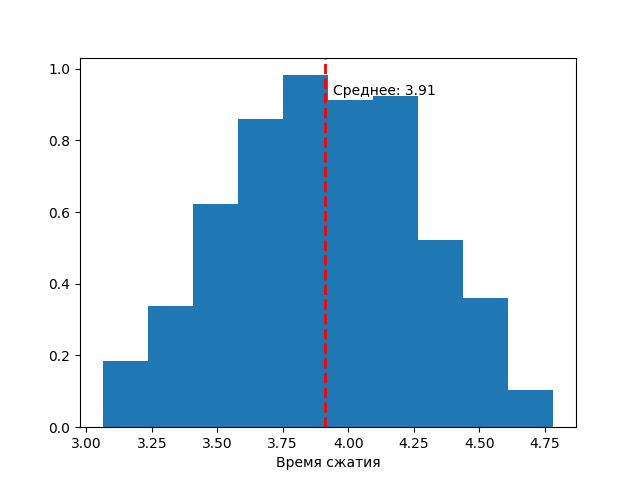
\includegraphics{images/hist-handmade-c-dev.png}
    \end{adjustbox}
    \caption{Время сжатия разработанным с нуля C-устройством.}\label{fig:hist-handmade-c-dev}
\end{figure}

{\tiny
\setlength\LTleft{-1.2cm}
    \begin{longtable}{|c|c|c|c|c|c|c|c|c|c|c|c|c|c|c|c|c|c|c|c|}%
        \caption{Время сжатия разработанным с нуля C-устройством.}\label{tbl:hist-handmade-c-dev} \\
        \hline
        № & $T$ &
        № & $T$ &
        № & $T$ &
        № & $T$ &
        № & $T$ &
        № & $T$ &
        № & $T$ &
        № & $T$ &
        № & $T$ &
        № & $T$ \\
        \hline
        \csvreader[column count=22,
                   no head,
                   table head=\hline,
                   late after line =\\\hline]{handmade-c-dev.csv}{
        1=\one, 2=\two, 3=\three, 4=\four,
        5=\five, 6=\six, 7=\seven, 8=\eight,
        9=\nine, 10=\ten, 11=\eleven, 12=\twelve,
        13=\thirteen, 14=\fourteen, 15=\fifteen, 16=\sixteen,
        17=\seventeen, 18=\eighteen, 19=\nineteen, 20=\twenty
        }
        {
            \one & \two &
            \three & \four &
            \five & \six &
            \seven & \eight &
            \nine & \ten &
            \eleven & \twelve &
            \thirteen & \fourteen &
            \fifteen & \sixteen &
            \seventeen & \eighteen &
            \nineteen & \twenty
        }
    \end{longtable}
}

\begin{figure}[!htbp]
    \centering
    \begin{adjustbox}{max totalsize={0.8\textwidth}{\textheight}}
        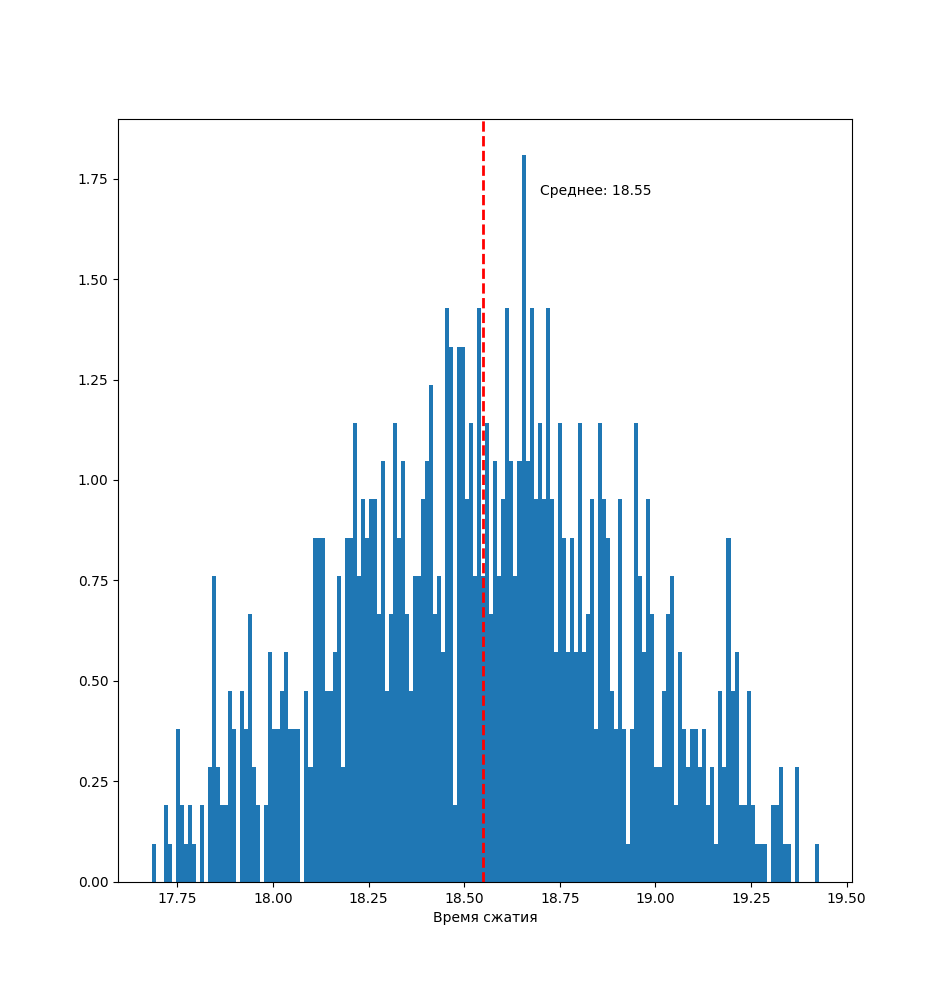
\includegraphics{images/hist-handmade-py-dev.png}
    \end{adjustbox}
    \caption{Время сжатия разработанным с нуля Python-устройством.}\label{fig:hist-handmade-py-dev}
\end{figure}

{\tiny
\setlength\LTleft{-1.5cm}
    \begin{longtable}{|c|c|c|c|c|c|c|c|c|c|c|c|c|c|c|c|c|c|c|c|}%
        \caption{Время сжатия разработанным с нуля Python-устройством.}\label{tbl:hist-handmade-py-dev} \\
        \hline
        № & $T$ &
        № & $T$ &
        № & $T$ &
        № & $T$ &
        № & $T$ &
        № & $T$ &
        № & $T$ &
        № & $T$ &
        № & $T$ &
        № & $T$ \\
        \hline
        \csvreader[column count=22,
                   no head,
                   table head=\hline,
                   late after line =\\\hline]{handmade-py-dev.csv}{
        1=\one, 2=\two, 3=\three, 4=\four,
        5=\five, 6=\six, 7=\seven, 8=\eight,
        9=\nine, 10=\ten, 11=\eleven, 12=\twelve,
        13=\thirteen, 14=\fourteen, 15=\fifteen, 16=\sixteen,
        17=\seventeen, 18=\eighteen, 19=\nineteen, 20=\twenty
        }
        {
            \one & \two &
            \three & \four &
            \five & \six &
            \seven & \eight &
            \nine & \ten &
            \eleven & \twelve &
            \thirteen & \fourteen &
            \fifteen & \sixteen &
            \seventeen & \eighteen &
            \nineteen & \twenty
        }
    \end{longtable}
}


\begin{figure}[!htbp]
    \centering
    \begin{adjustbox}{max totalsize={0.8\textwidth}{\textheight}}
        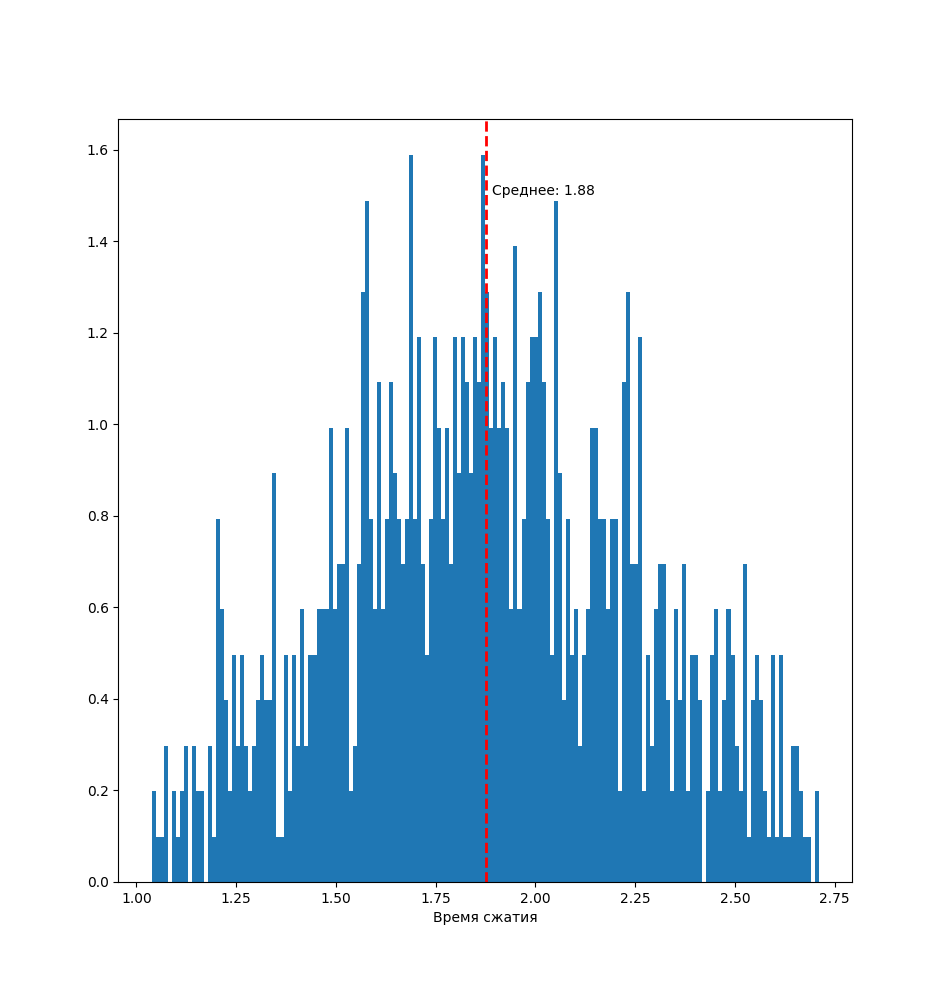
\includegraphics{images/hist-lib-c-dev.png}
    \end{adjustbox}
    \caption{Время сжатия C-устройством, использующим библиотеку сжатия.}\label{fig:hist-lib-c-dev}
\end{figure}

{\tiny
\setlength\LTleft{-1.2cm}
    \begin{longtable}{|c|c|c|c|c|c|c|c|c|c|c|c|c|c|c|c|c|c|c|c|}%
        \caption{Время сжатия C-устройством, использующим библиотеку сжатия.}\label{tbl:hist-lib-c-dev} \\
        \hline
        № & $T$ &
        № & $T$ &
        № & $T$ &
        № & $T$ &
        № & $T$ &
        № & $T$ &
        № & $T$ &
        № & $T$ &
        № & $T$ &
        № & $T$ \\
        \hline
        \csvreader[column count=22,
                   no head,
                   table head=\hline,
                   late after line =\\\hline]{lib-c-dev.csv}{
        1=\one, 2=\two, 3=\three, 4=\four,
        5=\five, 6=\six, 7=\seven, 8=\eight,
        9=\nine, 10=\ten, 11=\eleven, 12=\twelve,
        13=\thirteen, 14=\fourteen, 15=\fifteen, 16=\sixteen,
        17=\seventeen, 18=\eighteen, 19=\nineteen, 20=\twenty
        }
        {
            \one & \two &
            \three & \four &
            \five & \six &
            \seven & \eight &
            \nine & \ten &
            \eleven & \twelve &
            \thirteen & \fourteen &
            \fifteen & \sixteen &
            \seventeen & \eighteen &
            \nineteen & \twenty
        }
    \end{longtable}
}

\begin{figure}[!htbp]
    \centering
    \begin{adjustbox}{max totalsize={0.8\textwidth}{\textheight}}
        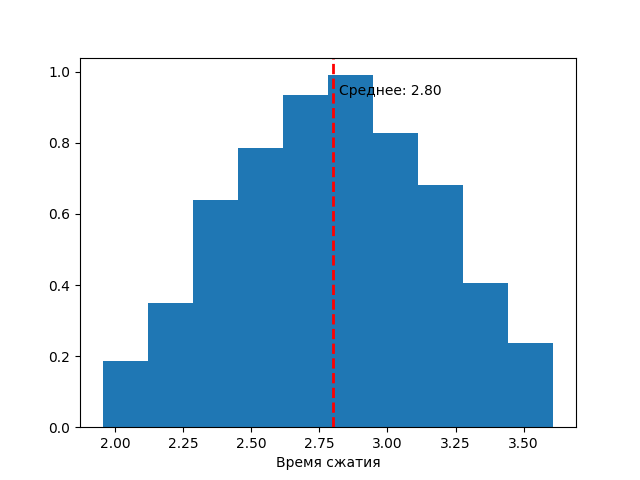
\includegraphics{images/hist-lib-py-dev.png}
    \end{adjustbox}
    \caption{Время сжатия Python-устройством, использующим библиотеку сжатия.}\label{fig:hist-lib-py-dev}
\end{figure}

{\tiny
\setlength\LTleft{-1.5cm}
    \begin{longtable}{|c|c|c|c|c|c|c|c|c|c|c|c|c|c|c|c|c|c|c|c|}%
        \caption{Время сжатия Python-устройством, использующим библиотеку сжатия.}\label{tbl:hist-lib-py-dev} \\
        \hline
        № & $T$ &
        № & $T$ &
        № & $T$ &
        № & $T$ &
        № & $T$ &
        № & $T$ &
        № & $T$ &
        № & $T$ &
        № & $T$ &
        № & $T$ \\
        \hline
        \csvreader[column count=22,
                   no head,
                   table head=\hline,
                   late after line =\\\hline]{lib-py-dev.csv}{
        1=\one, 2=\two, 3=\three, 4=\four,
        5=\five, 6=\six, 7=\seven, 8=\eight,
        9=\nine, 10=\ten, 11=\eleven, 12=\twelve,
        13=\thirteen, 14=\fourteen, 15=\fifteen, 16=\sixteen,
        17=\seventeen, 18=\eighteen, 19=\nineteen, 20=\twenty
        }
        {
            \one & \two &
            \three & \four &
            \five & \six &
            \seven & \eight &
            \nine & \ten &
            \eleven & \twelve &
            \thirteen & \fourteen &
            \fifteen & \sixteen &
            \seventeen & \eighteen &
            \nineteen & \twenty
        }
    \end{longtable}
}


\begin{figure}[!htbp]
    \centering
    \begin{adjustbox}{max totalsize={0.8\textwidth}{\textheight}}
        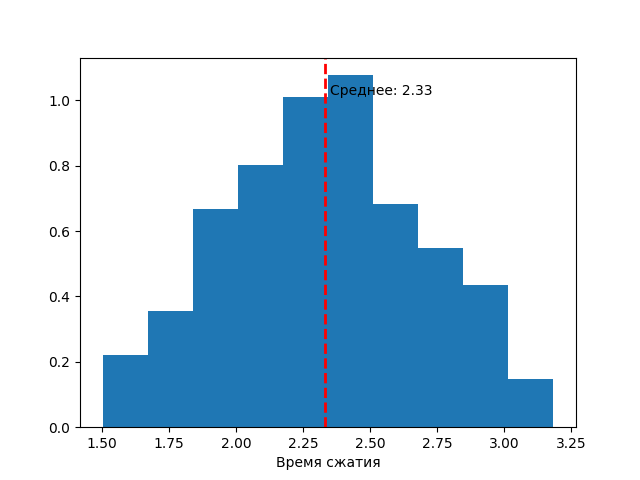
\includegraphics{images/hist-lib-c-network.png}
    \end{adjustbox}
    \caption{Время сжатия C-устройством по сети.}\label{fig:hist-lib-c-network}
\end{figure}


\begin{figure}[!htbp]
    \centering
    \begin{adjustbox}{max totalsize={0.8\textwidth}{\textheight}}
        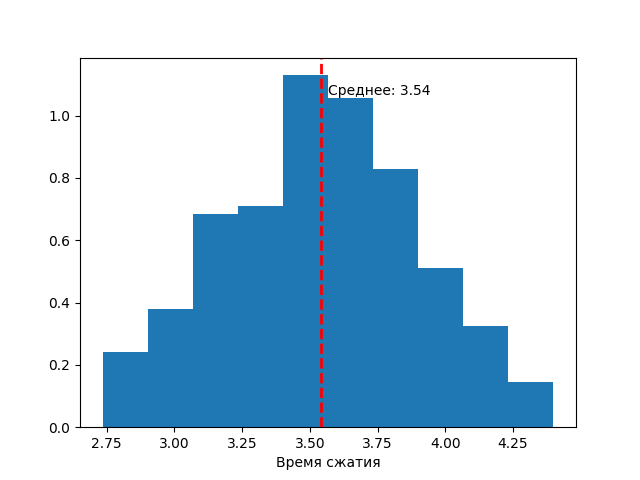
\includegraphics{images/hist-lib-py-network.png}
    \end{adjustbox}
    \caption{Время сжатия Python-устройством по сети.}\label{fig:hist-lib-py-network}
\end{figure}

\begin{figure}[!htbp]
    \centering
    \begin{adjustbox}{max totalsize={0.8\textwidth}{\textheight}}
        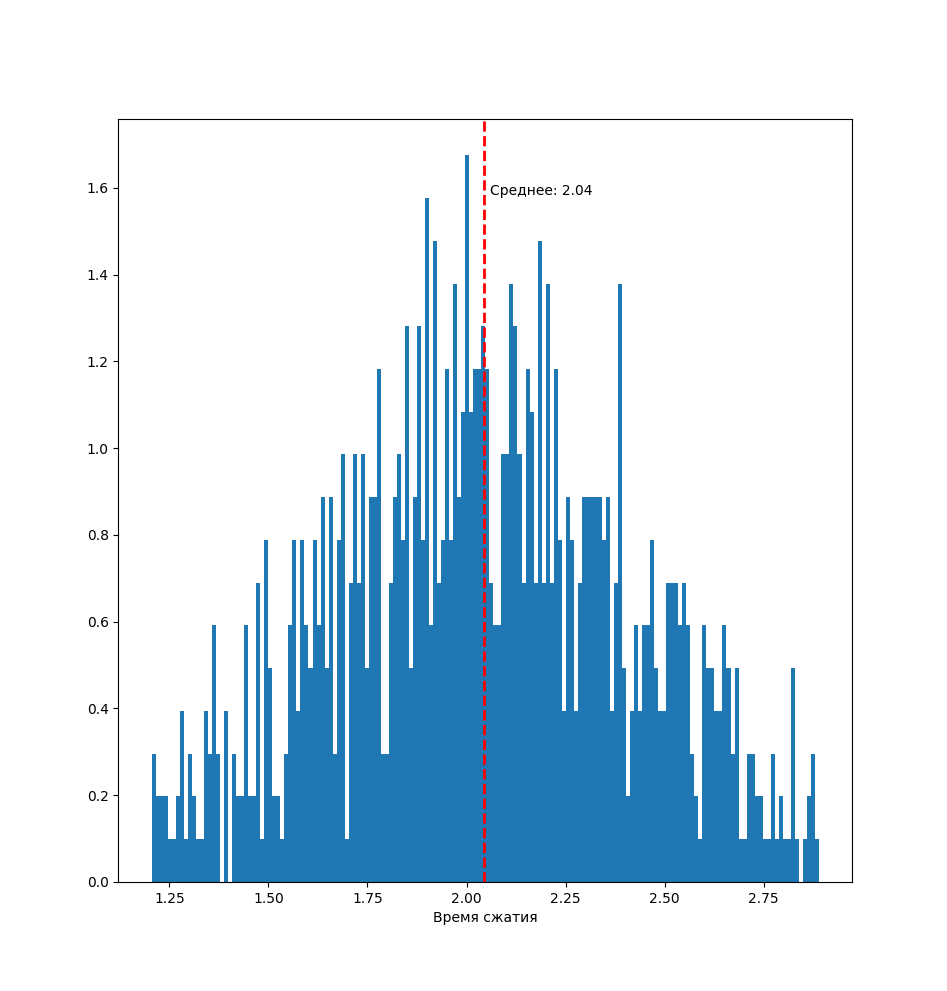
\includegraphics{images/hist-exec-c-dev.png}
    \end{adjustbox}
    \caption{Время сжатия C-устройством через подпроцесс.}\label{fig:hist-exec-c-dev}
\end{figure}

\begin{figure}[!htbp]
    \centering
    \begin{adjustbox}{max totalsize={0.8\textwidth}{\textheight}}
        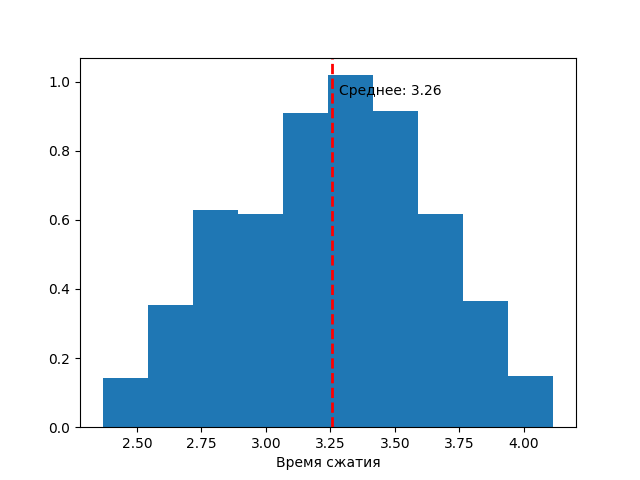
\includegraphics{images/hist-exec-py-dev.png}
    \end{adjustbox}
    \caption{Время сжатия Python-устройством через подпроцесс.}\label{fig:hist-exec-py-dev}
\end{figure}



\chapter{Программный код}\label{app:B}

Proof Of Concept реализация {\mylanguage}, \cref{lst:core.template.c,lst:main.py,lst:schema_parser.py}.

\begin{lstlisting}[language={C},basicstyle=\tiny,stepnumber=1,caption={Шаблон устройства},label={lst:core.template.c}]
#include "qemu/osdep.h"
#include "qapi/error.h"
#include "qom/object.h"
/*[[[cog
    import json as j
    import main as m

    with open(m.DEV_SCHEMA_FILE, 'r') as sf:
        SCHEMA = j.load(sf)

    device_header = SCHEMA["parent"]["header"]
    cog.outl(f'#include "{device_header}"')
   ]]]*/
/*[[[end]]]*/
#include "exec/address-spaces.h"
#include "hw/qdev-properties-system.h"

#include <Python.h>

#define IF_NULL_GOTO_ERR(VAR, BODY) \
    BODY; \
    if (!VAR){ \
        goto err; \
    }

#define PY_COMPILE_AND_GET_FUNC(FUNC_NAME, PY_CODE, PY_COMPILED, PY_MODULE, PY_FUNC) \
    if (!PY_COMPILED){ \
        IF_NULL_GOTO_ERR(PY_COMPILED, \
                         PY_COMPILED = Py_CompileString(PY_CODE, FUNC_NAME ".py", Py_single_input)) \
    } \
    IF_NULL_GOTO_ERR(PY_MODULE, \
                     PY_MODULE = PyImport_ExecCodeModule(FUNC_NAME "module", PY_COMPILED)) \
    IF_NULL_GOTO_ERR(PY_FUNC, \
                     PY_FUNC = PyObject_GetAttrString(PY_MODULE, FUNC_NAME))


typedef struct {
    char *name;
    size_t size;
} DeviceFieldMetaInfo;


/*[[[cog
    #
    # generating device class
    #

    import json as j
    import main as m
    from textwrap import indent, dedent
    INDENT = lambda s: indent(s, ' '*4)

    with open(m.DEV_SCHEMA_FILE, 'r') as sf:
        SCHEMA = j.load(sf)


    device_class    = m.get_device_class_name(SCHEMA, full = True)
    device_instance = m.get_device_class_name(SCHEMA)
    device_parent   = SCHEMA["parent"]["name"]


    cog.outl("typedef struct {")
    cog.outl(INDENT(f"{device_parent}Device parent_obj;"))
    cog.outl(f"}} {device_class};")
    cog.outl()
    cog.outl(f"typedef struct __attribute__((packed)) {{")
    for fname, ftype in m.get_nested_schema(SCHEMA, "device").items():
        cog.outl(INDENT(f"{ftype} {fname};"))
    cog.outl(f"}} {device_instance};")

    cog.outl()
    cog.outl()
    cog.outl(f"DeviceFieldMetaInfo device_fields[] = {{")
    for fname, ftype in m.get_nested_schema(SCHEMA, "device").items():
        cog.outl(INDENT(f'{{ "{fname}", sizeof({ftype}) }},'))
    cog.outl(INDENT('};'))
  ]]]*/
/*[[[end]]]*/

#define DEVICE_FIELDS_COUNT sizeof(device_fields)/sizeof(device_fields[0])

static PyObject* create_dict_for_class_fields(){
    PyObject* p_field_dicts[DEVICE_FIELDS_COUNT];
    PyObject *p_meta_info_aggregation = PyDict_New();
    for(int i = 0; i < DEVICE_FIELDS_COUNT; i++){
        int err = PyDict_Merge(p_meta_info_aggregation,
                               Py_BuildValue("{s:i}",
                                             device_fields[i].name,
                                             device_fields[i].size),
                               1);
        if(err){
            PyErr_Print();
            abort();
        }
    }
    return p_meta_info_aggregation;
}

PyObject *DictWithClassFields;

/*[[[cog
    #
    # generating device type
    #

    import json as j
    import main as m

    with open(m.DEV_SCHEMA_FILE, 'r') as sf:
        SCHEMA = j.load(sf)

    device_instance    = m.get_device_class_name(SCHEMA)
    device_name        = SCHEMA["name"]
    device_parent_type = SCHEMA["parent"]["type"]
    device_interface   = SCHEMA["parent"]["interface"]
    device_qtype       = SCHEMA["name"].upper()

    cog.outl(f'#define TYPE_{device_qtype} "{device_name}"')
    cog.outl(f"""OBJECT_DEFINE_TYPE_WITH_INTERFACES({device_instance},
                                       {device_name},
                                       {device_qtype},
                                       {device_parent_type}_DEVICE,
                                       {{ INTERFACE_{device_interface} }},
                                       {{ NULL }})""")
  ]]]*/
/*[[[end]]]*/

/*[[[cog
    #
    # generating function prototypes
    #

    import json as j
    import main as m
    from textwrap import indent, dedent
    INDENT = lambda s: indent(s, ' '*4)

    with open(m.DEV_SCHEMA_FILE, 'r') as sf:
        SCHEMA = j.load(sf)

    class_methods = SCHEMA["class"]["schema"]["methods"]
    class_init = m.create_device_method_proto(SCHEMA, "void", "class_init", "ObjectClass *oc, void *data")
    cog.outl(f"{class_init};")

    for method in class_methods:
        cog.outl(f'{m.create_device_method_proto(SCHEMA, method["c_ret"], method["c_name"], method["c_args"])};')
  ]]]*/
/*[[[end]]]*/

/*[[[cog
    #
    # generating device properties
    #

    import json as j
    import main as m
    from textwrap import indent, dedent
    INDENT = lambda s: indent(s, ' '*4)

    with open(m.DEV_SCHEMA_FILE, 'r') as sf:
        SCHEMA = j.load(sf)

    device_name = SCHEMA['name']

    cog.outl(f"static Property {device_name}_properties[] = {{")
    for p in m.get_nested_schema(SCHEMA, 'properties'):
        ptype         = p["type"].upper()
        pname         = f"\"{p['name']}\""
        pfield        = p["field"]
        dev_name      = m.get_device_class_name(SCHEMA)
        default_value = ''

        if "default_value" in p:
            default_value = ', ' + str(p["default_value"])

        cog.outl(INDENT(f"DEFINE_PROP_{ptype}({pname}, {dev_name}, {pfield}{default_value}),"))
    cog.outl(INDENT("DEFINE_PROP_END_OF_LIST()"))
    cog.outl("};")
  ]]]*/
/*[[[end]]]*/

/*[[[cog
    #
    # generating device MemoryRegionOps
    #

    import json as j
    import main as m
    from textwrap import indent, dedent
    INDENT = lambda s: indent(s, ' '*4)

    with open(m.DEV_SCHEMA_FILE, 'r') as sf:
        SCHEMA = j.load(sf)

    device_name = SCHEMA['name']

    for k,v in m.get_nested_schema(SCHEMA, "device").items():
        if v == "MemoryRegionOps":
            cog.outl(f"static const MemoryRegionOps {device_name}_mem_ops = {{")
            for mem_k, mem_v in SCHEMA["device"]["schema"][k].items():
                cog.outl(INDENT(f".{mem_k} = {mem_v},"))

            cog.outl(INDENT(f".read = {m.get_method_name(SCHEMA, 'read')},"))
            cog.outl(INDENT(f".write = {m.get_method_name(SCHEMA, 'write')},"))

            cog.outl("};")
  ]]]*/
/*[[[end]]]*/

/*[[[cog
    #
    # generating device and instance methods
    #

    import re
    import json as j
    import main as m

    from textwrap import indent, dedent
    INDENT = lambda s: indent(s, ' '*4)
    ALIGN_INDENT_BY = lambda s: ' ' * len(s)

    with open(m.DEV_SCHEMA_FILE, 'r') as sf:
        SCHEMA = j.load(sf)


    device_name      = SCHEMA["name"]
    class_init_proto = m.create_device_method_proto(SCHEMA, "void", "class_init", "ObjectClass *oc, void *data")

    cog.outl(f"{class_init_proto}{{")

    class_field_init = SCHEMA["class"]["schema"]["init"]["class_field_init"]

    if not any(filter(lambda cast: cast["dev_cast"]["type"] == "DeviceClass",
                      class_field_init)):
        default_dev_cast = {"dev_cast": {"type" : "DeviceClass", "cast": "DEVICE_CLASS"}}
        class_field_init = [default_dev_cast] + class_field_init

    for entry in class_field_init:
        cog.outl()
        dev_cast   = entry["dev_cast"]
        cast_type  = dev_cast['type']
        cast_macro = dev_cast['cast']

        cog.outl(INDENT(f"{cast_type} *{cast_type}_ptr = {cast_macro}(oc);"))

        for k,v in entry.items():
            if k == "dev_cast":
                continue
            cog.outl(INDENT(f"{cast_type}_ptr->{k} = {v};"))


    cog.outl(INDENT(f"device_class_set_props(DeviceClass_ptr, {device_name}_properties);"))

    cog.outl()
    cog.outl(INDENT(f'Py_SetProgramName("{device_name}");'))
    cog.outl(INDENT(f'Py_Initialize();'))
    cog.outl(INDENT(f'DictWithClassFields = create_dict_for_class_fields();'))
    cog.outl("}")
    cog.outl()
    cog.outl()

    for method in class_methods:
        method_proto = m.create_device_method_proto(SCHEMA, method["c_ret"], method["c_name"], method["c_args"])
        argc = method["c_args"].count(',') + 1
        arguments = [s.strip() for s in method["c_args"].split(',')]
        casts = [s.strip() for s in method["c_to_py_cast"].split(',')]

        argument_type_val = [arg.split() for arg in arguments]
        arguments_and_cast = list(zip(argument_type_val, casts))

        if len(argument_type_val) != len(arguments_and_cast):
            cog.error(f"{argument_type_val} and {casts} length mismatch!")

        cog.outl(f"{method_proto}{{")

        pass_args_to_python = ''
        memoryview_vars = []
        for i, (arg, cast) in enumerate(arguments_and_cast):
            is_pointer = '*' in arg[0] + arg[1]
            arg_val = arg[1].replace('*', '')
            if is_pointer:
                arg_val_as_buf = arg_val
            else:
                arg_val_as_buf= '&' + arg_val

            if method["c_name"] == "realize" and \
               "MemoryRegionOps" in m.get_nested_schema(SCHEMA, "device").values():
                device_fields = m.get_nested_schema(SCHEMA, "device")
                reverse_device_fields = dict(zip(device_fields.values(), device_fields.keys()))
                mem_io_field = reverse_device_fields["MemoryRegionOps"]
                cog.outl(INDENT(f"memory_region_init_io(&(({cast}*){arg_val_as_buf})->{mem_io_field},"))
                cog.outl(INDENT(f"                      OBJECT({arg_val_as_buf}),"))
                cog.outl(INDENT(f"                      &{device_name}_mem_ops,"))
                cog.outl(INDENT(f"                      {arg_val_as_buf},"))
                cog.outl(INDENT(f'                      "{device_name}-mmio",'))
                cog.outl(INDENT(f"                      1);"))

            memoryview_vars.append(f"p_mem_view_{arg_val}")
            pass_args_to_python += INDENT(INDENT(dedent(f"""
                                                 PyObject *p_mem_view_{arg_val} = PyMemoryView_FromMemory((char*){arg_val_as_buf},
                                                                                                 {ALIGN_INDENT_BY(arg_val)}sizeof({cast}),
                                                                                                 {ALIGN_INDENT_BY(arg_val)}PyBUF_WRITE);
                                                 if (!p_mem_view_{arg_val}){{
                                                     goto err;
                                                 }}
                                                 PyTuple_SetItem(p_func_args, {i}, p_mem_view_{arg_val});
                                                 """)))

            memoryview_vars_free = INDENT('\n'.join([f'Py_XDECREF({mv});' for mv in memoryview_vars]))
            py_return_code = ''
            py_return_val_name = ''
            if method["c_ret"] != "void":
                py_return_val_name = 'py_out'
                py_return_code = INDENT(dedent(f"""
                                        char *py_out_buf;
                                        {method["c_ret"]} {py_return_val_name};
                                        int ok = PyArg_ParseTuple(p_ret, "S", &py_out_buf);
                                        {py_return_val_name} = *({method["c_ret"]}*)py_out_buf;
                                        """))

        pass_args_to_python += INDENT(INDENT(f"PyTuple_SetItem(p_func_args, {argc}, DictWithClassFields);\n"))
        c_function_body = m.get_python_c_api_wrap(SCHEMA,
                                                  'class',
                                                  method["py_name"],
                                                  argc + 1,
                                                  pass_args_to_python,
                                                  return_val=py_return_val_name)
        if method["c_name"] == "finalize":
            err_handling_code = "if(Py_FinalizeEx()){\n" \
                                + INDENT(INDENT("PyErr_Print();\n")) \
                                + INDENT(INDENT("abort();\n")) \
                                + INDENT("}\n")
            c_function_body = re.sub("//.*?\n",
                                     err_handling_code + memoryview_vars_free + '\n',
                                     c_function_body)
        else:
            c_function_body = re.sub("\s+//.*?\n", f"\n{py_return_code}\n{memoryview_vars_free}\n", c_function_body, count=1)
            c_function_body = re.sub("\s+//.*?\n", f"\n{memoryview_vars_free}\n", c_function_body, count=1)
        c_function_body = '\n'.join(filter(lambda l: not re.match("\s+$", l), c_function_body.splitlines()))
        cog.outl(c_function_body)

        cog.outl("}")
        cog.outl()
        cog.outl()
  ]]]*/
/*[[[end]]]*/
\end{lstlisting}


\begin{lstlisting}[language={Python},basicstyle=\tiny,stepnumber=1,caption={Вспомогательные методы кодогенерации},label={lst:main.py}]
import os
import sys
import json
import inspect
import importlib.util
import subprocess as subp

from pathlib import Path
from textwrap import dedent

import schema_parser as sp


def get_nested_schema(schema: dict, key: str):
    return schema[key]['schema'][key]


def get_device_class_name(schema: dict, full=False):
    base_class_name = schema["name"].replace('_', ' ').title().replace(' ', '')
    if full:
        return base_class_name + "Class"
    return base_class_name


def get_function_text_from(sub_schema: dict, method_name: str):
    spec = importlib.util.spec_from_file_location("py_code", sub_schema["code"])
    py_code = importlib.util.module_from_spec(spec)
    spec.loader.exec_module(py_code)
    return inspect.getsource(getattr(py_code, method_name)).split('\n')


def get_python_c_api_wrap(schema: dict,
                          _from: str,
                          func_name: str,
                          tuple_size: int,
                          code_for_insert: str,
                          return_val: str = ''):
    c_char_source = [l + '\\n' for l in get_function_text_from(schema[_from], func_name)]

    py_code = f"static char *py_code = "
    py_code_start = len(py_code) + 8

    py_code += f'"{c_char_source[0]}"\n'
    for line in c_char_source[1:-1]:
        py_code += py_code_start*' ' + f'"{line}"\n'
    py_code += py_code_start*' ' + f'"{c_char_source[-1]}";'

    check_code = """if (!{what}){{
            goto err;
        }}"""

    return dedent(f"""
        {py_code}
        static PyObject *p_compiled_code = NULL;
        PyObject *p_module = NULL,
                 *p_func = NULL,
                 *p_func_args = NULL,
                 *p_ret = NULL;

        PY_COMPILE_AND_GET_FUNC("{func_name}",
                                py_code,
                                p_compiled_code,
                                p_module,
                                p_func);

        p_func_args = PyTuple_New({tuple_size});
        {check_code.format(what='p_func_args')}
        {code_for_insert}
        p_ret = PyObject_CallObject(p_func, p_func_args);
        {check_code.format(what='p_ret')}

        // for post creation code insert
        Py_XDECREF(p_module);
        Py_XDECREF(p_func);
        Py_XDECREF(p_func_args);
        Py_XDECREF(p_ret);
        return {return_val};

    err:
        PyErr_Print();
        // for post creation code insert
        Py_XDECREF(p_module);
        Py_XDECREF(p_func);
        Py_XDECREF(p_func_args);
        Py_XDECREF(p_ret);
        abort();
        """)


def get_method_name(schema: dict,
                    method_name: str):
    return f"{schema['name']}_{method_name}"


def create_device_method_proto(schema: dict,
                               ret_type: str,
                               method_name: str,
                               args: str,
                               static=True):
    method_proto = f"{ret_type} {get_method_name(schema, method_name)}({args})"
    if static:
        return f"static {method_proto}"
    return method_proto


DEV_SCHEMA_FILE = 'concrete_dev_schema.json'

if __name__ == '__main__':
    ENV = os.environ.copy()
    ENV["PYTHONPATH"] = Path('.').absolute()
    SCHEMA = sp.load_schema(sys.argv[1])

    with open(DEV_SCHEMA_FILE, 'w') as cds:
        json.dump(SCHEMA, cds, indent=2)


    subp.run(['cog', '-d', '-o', SCHEMA["name"] + '.c', sys.argv[2]],
             env=ENV)
\end{lstlisting}


\begin{lstlisting}[language={Python},basicstyle=\tiny,stepnumber=1,caption={Парсер схемы},label={lst:schema_parser.py}]
import json
import typing as t

from pathlib import Path


def load_schema(filename: str):
    schema_path = Path(filename)

    def get_load_path(path: Path):
        return path if path.is_absolute() else schema_path.parent / path

    def load_into_schema(schema_slice: dict,
                         key: str,
                         path: Path,
                         as_json=True):
        with open(path, 'r') as f:
            if as_json:
                schema_slice[key] = json.load(f)
            else:
                schema_slice[key] = f.read()


    with open(schema_path, 'r') as f:
        init_schema = json.load(f)
        for k in filter(lambda k: type(init_schema[k]) == dict and \
                                  'schema' in init_schema[k] and \
                                  'code' in init_schema[k], init_schema):
            subschema_path = get_load_path(Path(init_schema[k]['schema']))
            subschema_code = get_load_path(Path(init_schema[k]['code']))
            load_into_schema(init_schema[k], 'schema', subschema_path)
            init_schema[k]['code'] = str(subschema_code)

    return init_schema
\end{lstlisting}
      % Запасные слайды презентации
\end{document}
